% =====================================================================
% International Journal of Human-Computer Studies (Elsevier)
% Full draft -- DataGuard / The Auditability Gap
%
% Build:  pdflatex main && bibtex main && pdflatex main && pdflatex main
% =====================================================================
\documentclass[11pt,a4paper]{article}

% ----- Packages
\usepackage[utf8]{inputenc}
\usepackage[T1]{fontenc}
\usepackage{lmodern}
\usepackage{microtype}
\usepackage[margin=2.4cm]{geometry}
\usepackage{graphicx}
\usepackage{xcolor}
\usepackage{booktabs}
\usepackage{array}
\usepackage{multirow}
\usepackage{caption}
\usepackage{subcaption}
\usepackage{enumitem}
\usepackage{tikz}
\usepackage{pgfplots}
\usepackage{amsmath,amssymb}
\usepackage{url}
\usepackage[hidelinks]{hyperref}
\usepackage[round]{natbib}
\bibliographystyle{plainnat}  % switch to elsarticle-harv on submission

\pgfplotsset{compat=1.18}
\usetikzlibrary{arrows.meta,positioning,shapes.geometric,fit,calc,
                patterns,backgrounds,decorations.pathreplacing,shadows,
                shapes.symbols,shapes.misc}

% ----- Color palette (consistent across all TikZ figures)
\definecolor{dgBlue}    {RGB}{ 39, 99,178}
\definecolor{dgBlueL}   {RGB}{218,232,248}
\definecolor{dgBlueXL}  {RGB}{235,243,253}
\definecolor{dgOrange}  {RGB}{226,123, 32}
\definecolor{dgOrangeL} {RGB}{252,229,205}
\definecolor{dgOrangeXL}{RGB}{254,244,232}
\definecolor{dgGreen}   {RGB}{ 84,156, 84}
\definecolor{dgGreenL}  {RGB}{225,243,217}
\definecolor{dgGreenXL} {RGB}{240,250,235}
\definecolor{dgPurple}  {RGB}{132, 76,162}
\definecolor{dgPurpleL} {RGB}{233,221,242}
\definecolor{dgPurpleXL}{RGB}{246,239,250}
\definecolor{dgRed}     {RGB}{200, 64, 64}
\definecolor{dgRedL}    {RGB}{248,215,218}
\definecolor{dgTeal}    {RGB}{ 38,140,140}
\definecolor{dgTealL}   {RGB}{211,236,236}
\definecolor{dgGold}    {RGB}{218,165, 32}
\definecolor{dgGoldL}   {RGB}{251,236,196}
\definecolor{dgGrey}    {RGB}{ 90, 90, 90}
\definecolor{dgGreyL}   {RGB}{235,235,235}
\definecolor{dgNavy}    {RGB}{ 28, 60,108}
\definecolor{dgRose}    {RGB}{215, 95,140}
\definecolor{dgRoseL}   {RGB}{247,224,233}

% ----- Title block
\title{\bfseries The Auditability Gap: \\
A Human-Centered Study of Privacy-Label Verification \\
in the Google Play Data Safety Ecosystem}
\author{Anonymous Author(s)\\\small (Submitted to the International Journal of
Human-Computer Studies)}
\date{}

% ----- Macros
\newcommand{\dataguard}{\textsc{DataGuard}}
\newcommand{\dgrule}[1]{\textsf{R#1}}

\begin{document}
\maketitle

\begin{abstract}
\noindent
Mobile-app privacy labels promise transparency by translating complex data
practices into compact, scannable tables. But the public value of such labels
depends on a property that has been almost entirely absorbed into the broader
notion of accuracy: whether the label can be \emph{audited} against the app's
own privacy policy by a motivated human reviewer. We introduce
\emph{auditability} as a first-class human-computer-interaction (HCI) property
of structured privacy disclosures, distinguish it from \emph{readability} and
from automated \emph{accuracy}, and study it empirically in the Google Play
Data Safety ecosystem. We built \dataguard, an evidence-oriented audit
interface that displays a parsed Data Safety disclosure alongside extracted
privacy-policy passages, and we collected $1{,}506$ human audit judgments
across $1{,}214$ unique Android apps in $12$ Google Play categories produced by
seven trained annotators. Annotators marked Data Safety \emph{sharing}
disclosures as incorrect in $41.3\%$ of non-empty judgments and as incomplete
in $39.8\%$; \emph{collection} disclosures were judged incorrect in $41.1\%$
and incomplete in $44.6\%$. At least one defect was recorded for $79.0\%$ of
the $1{,}214$ audited apps, with category-level defect rates ranging from
$28.8\%$ (Shopping) to $54.7\%$ (Business) on the per-category
average across the four judgment axes. Apps whose label declared
\emph{no} sharing or \emph{no} collection were the worst case, not the safest:
non-empty audit judgments flagged $46.8\%$ of no-shared and $59.6\%$ of
no-collected labels as incorrect. Inter-annotator agreement on the $286$
doubly-labeled apps was low (Cohen's $\kappa$ from $-0.11$ to $0.17$) and
lowest for completeness, indicating that audit difficulty reflects interpretive
ambiguity rather than annotator inattention. A lexical scoping of $1{,}441$
free-text rationale records surfaces four recurring sources of ambiguity ---
third-party services, generic legal hedging, device identifiers, and no-data
contradictions --- which we recast as four interface requirements for
evidence-grounded audit. We position \dataguard{} as a reusable research
instrument and contribute (i)~the auditability-gap framework, (ii)~a public
audit-judgment dataset of unprecedented scale and depth, (iii)~statistical
evidence that the gap is large, category-dependent, and interpretive, and
(iv)~four design guidelines that pivot privacy interfaces from
\emph{showing labels} toward \emph{showing evidence}.
\end{abstract}

\noindent\textbf{Keywords:}\ privacy labels; Data Safety; auditability;
privacy policy; Android; mobile privacy; usable privacy; human--AI review;
evidence-grounded interfaces; transparency.

\bigskip
\hrule
\bigskip

% =====================================================================
\section{Introduction}
\label{sec:intro}
% =====================================================================
A modern Android app discloses its data practices through two coexisting,
asymmetric channels. The first is the \emph{Google Play Data Safety} section:
a structured, developer-declared table that lists data types collected and
shared, alongside processing purposes and security
practices~\citep{googledatasafety2022}. The second is the free-form
\emph{privacy policy}, a long, legally drafted document with no fixed schema
and no platform-imposed
taxonomy~\citep{mcdonald2008cost,fabian2017large,jensen2004privacy}. Users
encounter both. Regulators rely on both. Any meaningful claim of transparency
rests on the assumption that the two channels are \emph{consistent}---that a
reader who reaches for the supporting evidence will, in fact, find it.

A large body of HCI work has asked whether such labels are \emph{readable}
---can a user scan the table and infer what an app
does~\citep{kelley2009nutrition,kelley2010standardizing,schaub2015design,
cranor2012necessary}? A parallel security-and-systems literature has asked
whether they are \emph{accurate}---can an automated pipeline confirm that
label claims match observed app behaviour or NLP-extracted policy
clauses~\citep{andow2019policylint,andow2020policheck,zimmeck2019maps,
xiao2023lalaine,khandelwal2024unpacking,harkous2018polisis}? We argue that
a third property has received almost no attention as a problem in its own
right: \emph{auditability}. Auditability asks whether a \emph{human reviewer}
can, using the materials a regulator or motivated user would actually have at
hand, decide whether a label is supported by the policy. A label can be
perfectly readable, and yet impossible to audit, when the supporting evidence
is buried in vague language that uses a different vocabulary from the platform
schema, refers to ecosystem actors the schema cannot name, or hedges its
claims so heavily that any binary verdict is forced.

\paragraph{The auditability gap.}
We define the \emph{auditability gap} as the cognitive distance an HCI user
must traverse when one channel (a label) is structured into a fixed taxonomy
of categories, types, purposes and optionality flags, and the other channel
(a policy) is a long natural-language document organised around legal
boilerplate, ecosystem actors and exception clauses. The gap is not a
property of either channel alone; it emerges from the \emph{mapping} between
them. A no-data claim is the limiting case: a Data Safety label that reports
\emph{no shared data} is trivially readable, yet is materially contradicted
whenever the policy mentions analytics SDKs, advertising IDs or third-party
service providers. Closing this gap is a human-computer-interaction problem
because its difficulty is rooted in document representation, interface
layout and the cognitive economics of cross-document comparison, all of which
sit squarely in the domain of HCI design.

\paragraph{Approach.}
We approached auditability empirically. We built \dataguard, an audit
interface that lets a trained annotator inspect a parsed Data Safety panel
and an extracted privacy-policy panel side by side, then record four
judgments per app: (i)~sharing correctness, (ii)~sharing completeness,
(iii)~collection correctness, and (iv)~collection completeness, together
with free-text rationale and the policy fragment used as evidence. We
crawled $2{,}400$ Google-Play apps balanced across $12$ categories, parsed
$3{,}576$ Data Safety records, and collected $1{,}506$ judgments over
$1{,}214$ unique apps from seven trained annotators (one PhD-level computer
scientist; six advanced software-engineering, AI and information-assurance
students). We then analysed the resulting corpus along four axes:
disclosure landscape, per-app judgment, inter-annotator agreement, and the
rationale text that explains \emph{why} a judgment was made.

\paragraph{Why now.}
Three convergent forces make this an opportune moment for an
auditability-centred study. First, structured platform labels are now
mature artefacts: Google's Data Safety section, launched in $2022$,
covers the entire Play store and has been the subject of multiple
large-scale measurement
studies~\citep{khandelwal2024unpacking,khandelwal2023comparing}. Second,
the regulatory environment has shifted: privacy-disclosure obligations
under the GDPR, CCPA/CPRA, and adjacent statutes are now being
operationalised against precisely the kind of structured label our work
audits, and the question ``what does the label commit the developer
to?'' is becoming legally consequential rather than merely informative.
Third, recent advances in large-language-model-based document
comprehension---particularly evidence-grounded retrieval-augmented
question answering over policy
text~\citep{ravichander2019question,ahmad2021intent}---make it plausible
that an interface like \dataguard{} can be augmented with an AI
assistant in the near term. The risk is that the assistant will be
deployed before its evidence-grounding quality has been validated; the
present study provides exactly the empirical baseline against which
such an assistant must be measured.

\paragraph{Findings.}
Four results stand out. First, audit defects are pervasive but
\emph{strongly category-dependent}: $79.0\%$ of audited apps had at
least one defect, and the per-category average across the four
judgment axes ranges from $28.8\%$ (Shopping) to $54.7\%$ (Business),
suggesting that auditability is shaped by app category
rather than being uniformly random. Second, apps that label themselves as
having \emph{no} data flow are the worst audit case, not the safest:
$46.8\%$ of non-empty audit judgments on no-sharing labels and $59.6\%$ on
no-collection labels were marked incorrect. Third, when two annotators
reviewed the same app, Cohen's $\kappa$ never exceeded $0.17$ and was
lowest for completeness ($-0.11$); the agreement signal is not noise but
evidence that the task is genuinely interpretive. Fourth, $95.7\%$ of
judgments carried a free-text rationale, and a lexical scoping of those
rationales identified four recurring ambiguity sources: third-party
advertising/analytics ($54.5\%$), generic legal hedging ($44.7\%$), device
identifiers ($35.5\%$), and no-data contradictions ($30.4\%$). These four
themes become the entry points for our design guidelines.

\paragraph{Contributions.}
The paper makes four contributions:
\begin{enumerate}[leftmargin=*,nosep,topsep=2pt]
  \item \textbf{Conceptual.} We introduce auditability as a distinct HCI
        property of structured privacy disclosures and define the
        auditability gap as the cross-document mapping problem between a
        platform taxonomy and a long-form policy
        (\S\ref{sec:related-work}--\ref{sec:concept}).
  \item \textbf{Methodological.} We release \dataguard{} as a reusable
        evidence-comparison instrument for studying privacy-disclosure
        auditing, alongside the audit-judgment schema and rationale
        protocol (\S\ref{sec:dataguard}).
  \item \textbf{Empirical.} We report the first large-scale, expert
        human-audit corpus of Google-Play Data Safety: $1{,}506$ judgments,
        $1{,}214$ apps, $12$ categories, with statistical tests of
        category-level variation and inter-annotator agreement
        (\S\ref{sec:study1}--\ref{sec:study4}).
  \item \textbf{Design.} We translate the four recurring rationale themes
        into four concrete interface requirements---evidence-first labels,
        ambiguity-aware review, taxonomy-mapping support, and third-party
        flow visibility---and sketch a controlled prospective user study
        capable of validating them (\S\ref{sec:design}--\ref{sec:future}).
\end{enumerate}

The remainder of the paper is structured as follows.
Section~\ref{sec:related-work} positions our work against prior research on
mobile privacy labels, policy comprehension and disclosure accountability.
Section~\ref{sec:concept} states the auditability-gap framework formally.
Section~\ref{sec:dataguard} describes \dataguard{} as a system and a
research instrument. Section~\ref{sec:data} describes our data assets and
annotator profile. Sections~\ref{sec:study1}--\ref{sec:study4} present the
four studies. Section~\ref{sec:design} derives interface requirements.
Section~\ref{sec:discussion} discusses implications and threats to
validity. Section~\ref{sec:future} sketches a prospective controlled study
and AI-quality measures, and Section~\ref{sec:conclusion} concludes.

% =====================================================================
\section{Background and Related Work}
\label{sec:related-work}
% =====================================================================
We separate prior work into four threads, then highlight the gap we
target.

\subsection{Privacy notices, comprehension, and the cost of reading}
Privacy law and HCI have long known that long-form privacy policies are not
read. \citet{mcdonald2008cost} estimated that a typical user encounters
hundreds of hours of unread policy text per year. Large-scale readability
studies of policies confirm that they are written at high reading levels and
are dominated by hedging and legal
boilerplate~\citep{fabian2017large,jensen2004privacy}. Empirical work has
repeatedly shown that users systematically misjudge what apps and websites
actually do with their data~\citep{rao2016expecting,acquisti2015privacy},
and that even attentive readers struggle to extract a binary commitment
from policy text shaped by lawyers rather than by interaction
designers~\citep{bhatia2016theory}.

\subsection{Privacy labels: readability and adoption}
The \emph{nutrition label} metaphor of~\citet{kelley2009nutrition} and
\citet{kelley2010standardizing} demonstrated that structured tables make
privacy disclosures faster to read and easier to compare than full-text
policies. \citet{schaub2015design} extended the analysis to a notice
design space. On mobile, \citet{felt2012android}
and~\citet{egelman2013choice} showed that Android permission notices were
largely ignored at install time and that the timing and granularity of
notices matter as much as their content. Permission and notice nudging
work, notably~\citet{almuhimedi2015your}, has shown that just-in-time
feedback about how often a user's data is being accessed can dramatically
shift their privacy behaviour. Personalised privacy assistants extend the
notice principle into a recommendation
loop~\citep{lin2014modeling,liu2016follow}. Platform labels operationalised
the readability work at scale: Apple's App Privacy Labels in
$2020$~\citep{appleprivacylabels2020} and Google's Data Safety section in
$2022$~\citep{googledatasafety2022} both adopted a structured-table format.
\citet{cranor2012necessary} cautioned, however, that standardised
disclosure mechanisms are necessary but not sufficient: a label is only as
valuable as the evidence trail that backs it. Our work treats these labels
as the \emph{readable} channel that auditability problems then attach to.

\subsection{Disclosure accountability: automated mismatch analysis}
A parallel security literature has used NLP and dynamic-analysis pipelines
to test whether disclosures are correct. \emph{Polisis} extracts
fine-grained data practices from policies using deep
learning~\citep{harkous2018polisis}. \emph{PolicyLint} identifies internal
contradictions within a single policy by considering negation and semantic
levels of data objects, and reported $14.2\%$ of $11{,}430$ Google-Play
policies as contradictory~\citep{andow2019policylint}.
\emph{PoliCheck} extended this analysis to entity-sensitive
flow-to-policy checks and found that up to $42.4\%$ of $13{,}796$ apps
either incorrectly disclose or fail to disclose sensitive
flows~\citep{andow2020policheck}. \emph{MAPS} scaled compliance analysis to
a million apps~\citep{zimmeck2019maps,zimmeck2017automated}. For platform
labels specifically, \citet{xiao2023lalaine}'s \emph{Lalaine} audited
$5{,}102$ iOS apps and detected $3{,}423$ Apple-label non-compliance
instances; \citet{khandelwal2024unpacking} measured $1.1\,$M Google-Play
Data Safety entries and interviewed developers;
\citet{khandelwal2023comparing} cross-compared Android and iOS labels for
$1{,}703$ matched apps; \citet{li2022understanding} surfaced the
developer-side challenge of filling in nutrition labels accurately. At the
runtime side, \citet{reardon2019fifty} and~\citet{reyes2018wont} documented
how Android apps circumvent the permissions system or leak children's data;
\citet{razaghpanah2018apps} and~\citet{ren2018bug} extended the same
analysis to longitudinal and tracker-level studies of the mobile
ecosystem; \citet{englehardt2016online} characterised web-scale tracking
behaviour at the same magnitude. \emph{Crucially, all of this work
proceeds without a human in the loop.} It assumes that the auditor is an
analyser, not a person.

\subsection{Annotation, ambiguity and evidence-grounded review}
A third line of work treats privacy policies as a corpus for human
annotation. The OPP-115 corpus established a fine-grained schema for $115$
website policies annotated by ten legal-trained
graduate students~\citep{wilson2016creation};
\citet{sathyendra2017identifying} extended it to user-choice provisions,
and~\citet{ravichander2019question} formalised question-answering as a
benchmark for privacy-policy comprehension.
\citet{bhatia2016theory} formalised a theory of vagueness in privacy text;
\citet{breaux2014eddy} introduced a formal language to specify and analyse
data-flow rules; \citet{slavin2016toward} mapped policy text to Android
source code to detect privacy-policy violations;
and~\citet{ahmad2021intent} cast policy comprehension as intent
classification and slot filling. On the consumer-contract side,
\emph{CLAUDETTE} pioneered evidence-grounded flagging of unfair clauses in
terms-of-service documents~\citep{lippi2019claudette}. On the human-AI
side, \citet{amershi2019guidelines} synthesised human-AI interaction
guidelines; \citet{cai2019hello} and~\citet{liao2020questioning}
stressed that AI assistance should surface evidence \emph{before}
suggesting decisions; and \citet{bansal2021does} showed that
unexplained AI outputs can degrade complementary team performance.
The contextual-integrity framework
of~\citet{nissenbaum2004privacy} is a precedent for treating contextual
appropriateness as a designable property of disclosure. Together these
works show that ambiguity is a \emph{structural} property of privacy
text, not an artefact of annotator quality.

\subsection{Cross-platform precedents and developer-side challenges}
A small but rapidly growing literature compares structured label
ecosystems across platforms and across stakeholders. Direct comparison
of $1{,}703$ apps that ship on both stores~\citep{khandelwal2023comparing}
showed that the very same app can present materially different label
content on Android and iOS, despite the underlying app behaviour being
near-identical---an explicit auditability problem at the platform
boundary. On the developer side, \citet{li2022understanding} interviewed
practitioners filling in Apple's privacy labels and found that
``compliance via guesswork'' is the modal experience: developers were
unsure which taxonomy category a given third-party SDK should map to,
defaulted to under-disclosure, and often relied on the SDK vendor's
own disclosures rather than auditing the runtime behaviour of their
app. \citet{khandelwal2024unpacking} extended the same line of analysis
to $1.1$M Data Safety entries on Google Play and again documented broad
declarative under-disclosure relative to the policy text. We add the
\emph{reviewer}-side perspective to that triangle: even motivated
trained human reviewers, given the platform label and the policy, find
the audit ambiguous.

\subsection{Where the gap sits}
Figure~\ref{fig:gap-positioning} shows the conceptual position of our
contribution. Readability research treats the label as the unit of
analysis; accuracy research treats the policy (or app binary) as the unit
of analysis; we treat the \emph{mapping} between them as the unit, and we
treat the \emph{human reviewer} as the limiting subject. Auditability is
the leg of the triangle that has not yet been instrumented.

% --- Figure: positioning
\begin{figure}[t]
\centering
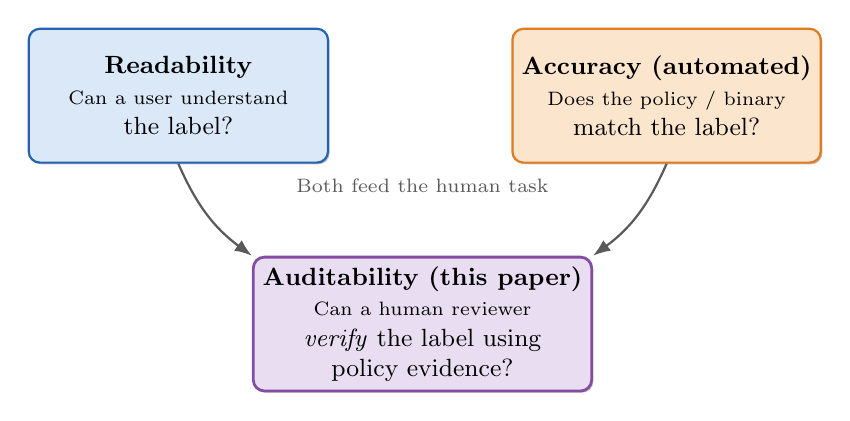
\begin{tikzpicture}[
  >={Latex[length=2.2mm]},
  every node/.style={font=\small},
  prop/.style={draw=dgGrey,thick,rounded corners=4pt,minimum width=3.8cm,
               minimum height=1.7cm,align=center,
               drop shadow={shadow xshift=0.6pt,shadow yshift=-0.6pt}},
  ours/.style={prop,fill=dgPurpleL,draw=dgPurple,line width=1pt}
]
\node[prop,fill=dgBlueL,draw=dgBlue] (read) at (0,0)
   {\textbf{Readability}\\\scriptsize Can a user understand\\the label?};
\node[prop,fill=dgOrangeL,draw=dgOrange] (acc) at (6.2,0)
   {\textbf{Accuracy (automated)}\\\scriptsize Does the policy / binary\\match the label?};
\node[ours] (audit) at (3.1,-2.9)
   {\textbf{Auditability (this paper)}\\\scriptsize Can a human reviewer\\\emph{verify} the label using\\policy evidence?};
\draw[->,dgGrey,thick] (read.south) to[bend right=15] (audit.north west);
\draw[->,dgGrey,thick] (acc.south)  to[bend left=15]  (audit.north east);
\node[font=\scriptsize,dgGrey] at (3.1,-1.15)
   {Both feed the human task};
\end{tikzpicture}
\caption{Conceptual position of the present paper. Readability work
studies the label; accuracy work studies the policy or app behaviour;
the auditability gap lives in the human mapping between them.}
\label{fig:gap-positioning}
\end{figure}

% =====================================================================
\section{The Auditability Gap and DataGuard}
\label{sec:framework}
% =====================================================================
\subsection{The auditability gap as a measurable HCI property}
\label{sec:concept}
% =====================================================================
We treat \emph{auditability} as a property of a pair of disclosures
$(\ell, p)$, where $\ell$ is a structured label drawn from a finite
schema $\mathcal{S}_{\ell}$ and $p$ is a free-form policy text drawn from
the open vocabulary~$\mathcal{V}_{p}$. An audit is a function
$a : (\ell, p, \mathcal{H}) \to \{\textsc{ok}, \textsc{contradict},
\textsc{omit}, \textsc{ambig}\}$, where $\mathcal{H}$ stands for the
hypotheses, training and time budget that the human reviewer brings to the
task. We say the pair $(\ell, p)$ is \emph{auditable} when an attentive
human reviewer can reach a stable verdict with reasonable effort, and we
define the \emph{auditability gap} as the increase in cognitive cost
introduced by the mismatch between $\mathcal{S}_{\ell}$ and
$\mathcal{V}_{p}$.

\paragraph{Why this is different from accuracy.}
Automated accuracy analyses fix $\mathcal{H}$ implicitly: the analyser uses
a classifier trained on a fixed taxonomy, runs deterministically, and
records its verdict. Auditability is the \emph{human} version of the same
question: the same $(\ell, p)$ pair, presented through some interface
$\mathcal{I}$, must yield a stable verdict in the head of a human reviewer.
The auditability gap therefore depends on three factors: (i)~the schema
distance between $\mathcal{S}_{\ell}$ and $\mathcal{V}_{p}$,
(ii)~the interface design $\mathcal{I}$ that mediates the comparison, and
(iii)~the cognitive resources $\mathcal{H}$ of the reviewer. Items (i) and
(iii) are out of designer's reach in any individual app; item (ii) is the
HCI lever.

\paragraph{Why this is different from readability.}
Readability indexes only the label. A label that says ``no shared data''
is maximally readable: it has one token and one bit of information. Its
auditability, however, is precisely the situation in which it is most
likely to fail---the policy will almost always mention \emph{some}
data practice that contradicts an absolute negative claim.

\paragraph{Four failure modes.}
We can taxonomise the failure of $(\ell, p)$ along the four corners of an
audit. Figure~\ref{fig:failure-modes} shows them. \textsc{Contradict}: the
policy contains a statement whose data type, purpose or recipient is
inconsistent with the structured claim. \textsc{Omit}: the policy
references a data practice that has no corresponding structured claim.
\textsc{Ambig}: the policy uses a generic legal hedge, a third-party
reference or an identifier vocabulary that does not map cleanly onto the
schema. \textsc{Ok}: every claim in $\ell$ is supported by, and every
practice in $p$ is reflected in, the structured table. The bulk of the
present paper documents that, in practice, \textsc{Ok} is far from the
modal outcome.

% --- Figure: failure modes (2x2; axis name separated from Pass/Fail level)
\begin{figure}[t]
\centering
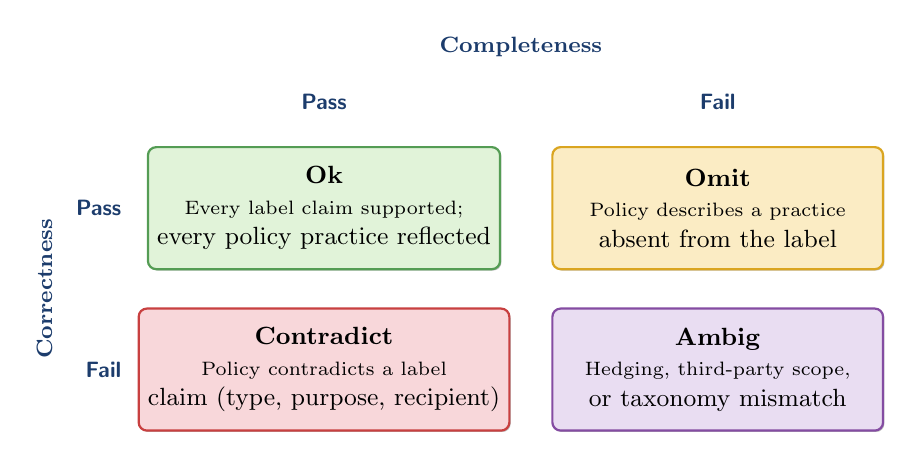
\begin{tikzpicture}[
  every node/.style={font=\small},
  cell/.style={draw,thick,align=center,minimum width=4.2cm,
               minimum height=1.55cm,rounded corners=3pt,
               drop shadow={shadow xshift=0.5pt,shadow yshift=-0.5pt}},
  ok/.style   ={cell,fill=dgGreenL,draw=dgGreen},
  cont/.style ={cell,fill=dgRedL,draw=dgRed},
  omit/.style ={cell,fill=dgGoldL,draw=dgGold},
  amb/.style  ={cell,fill=dgPurpleL,draw=dgPurple},
  axname/.style={font=\footnotesize\bfseries,text=dgNavy},
  level/.style={font=\footnotesize\bfseries,text=dgNavy}
]
% Column axis: top umbrella "Completeness" + level under it
\node[axname] at (2.5, 2.05)  {Completeness};
\node[level]  at (0,    1.35) {\textsf{Pass}};
\node[level]  at (5,    1.35) {\textsf{Fail}};
% Row axis: left umbrella "Correctness" (rotated) + Pass/Fail next to cells
\node[axname,rotate=90] at (-3.55,-1.025) {Correctness};
\node[level,anchor=east] at (-2.45, 0)    {\textsf{Pass}};
\node[level,anchor=east] at (-2.45,-2.05) {\textsf{Fail}};
% cells
\node[ok]   (ok)    at (0,0)
   {\textbf{\textsc{Ok}}\\\scriptsize Every label claim supported;\\every policy practice reflected};
\node[omit] (omit)  at (5,0)
   {\textbf{\textsc{Omit}}\\\scriptsize Policy describes a practice\\absent from the label};
\node[cont] (cont)  at (0,-2.05)
   {\textbf{\textsc{Contradict}}\\\scriptsize Policy contradicts a label\\claim (type, purpose, recipient)};
\node[amb]  (amb)   at (5,-2.05)
   {\textbf{\textsc{Ambig}}\\\scriptsize Hedging, third-party scope,\\or taxonomy mismatch};
\end{tikzpicture}
\caption{The four corners of a Data Safety / privacy-policy audit,
arranged as a $2{\times}2$ matrix over the correctness (rows) and
completeness (columns) axes. The lower-right \textsc{Ambig} cell
captures cases that resist a clean verdict on either axis.}
\label{fig:failure-modes}
\end{figure}

% =====================================================================
\subsection{\dataguard{}: an audit interface as research instrument}
\label{sec:dataguard}
% =====================================================================
\dataguard{} is the artefact that makes the audit task observable. It is
\emph{not} evaluated in this paper as a finished consumer tool. It is
used as a research instrument that operationalises label verification as
an interactive comparison task and records the resulting judgments,
rationales and evidence pointers.

\subsubsection{System architecture}
\label{subsec:architecture}
Figure~\ref{fig:architecture} shows the full architecture. The system
consists of an acquisition layer that scrapes Google Play, two structured
extractors that operate over Data Safety pages and policy URLs, a backing
data store, and an annotation web interface that orchestrates the audit
task. \dataguard{} was designed so that every piece of \emph{evidence} a
human reviewer might want during the audit is one click away from the
structured claim that depends on it.

% --- Figure: architecture (resized to fit text width exactly)
\begin{figure*}[t]
\centering
\resizebox{\textwidth}{!}{%
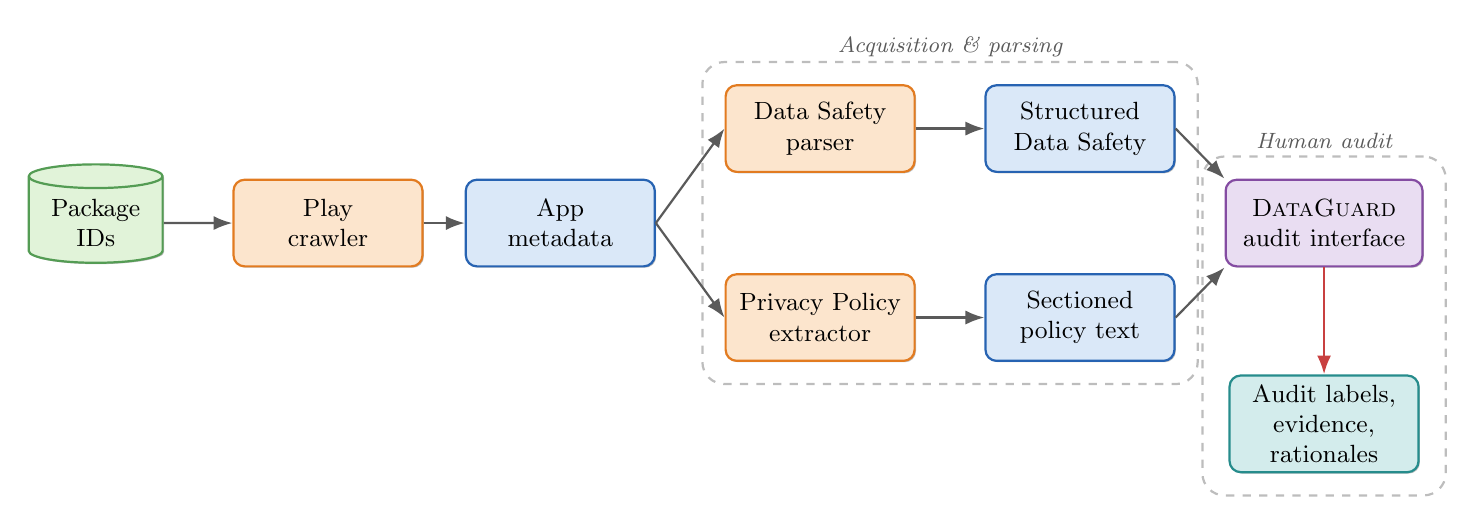
\begin{tikzpicture}[
  >={Latex[length=2.4mm]},
  every node/.style={font=\small},
  src/.style ={draw=dgBlue,fill=dgBlueL,rounded corners=4pt,thick,
               minimum width=2.4cm,minimum height=1.1cm,align=center,
               drop shadow={shadow xshift=0.5pt,shadow yshift=-0.5pt}},
  proc/.style={draw=dgOrange,fill=dgOrangeL,rounded corners=4pt,thick,
               minimum width=2.4cm,minimum height=1.1cm,align=center,
               drop shadow={shadow xshift=0.5pt,shadow yshift=-0.5pt}},
  store/.style={draw=dgGreen,fill=dgGreenL,thick,
                cylinder,shape border rotate=90,aspect=0.22,
                minimum width=1.7cm,minimum height=1.25cm,align=center,
                drop shadow={shadow xshift=0.5pt,shadow yshift=-0.5pt}},
  human/.style={draw=dgPurple,fill=dgPurpleL,rounded corners=4pt,thick,
                minimum width=2.5cm,minimum height=1.1cm,align=center,
                drop shadow={shadow xshift=0.5pt,shadow yshift=-0.5pt}},
  output/.style ={draw=dgTeal,fill=dgTealL,thick,rounded corners=4pt,
                minimum width=2.4cm,minimum height=1.1cm,align=center,
                drop shadow={shadow xshift=0.5pt,shadow yshift=-0.5pt}}
]
% Acquisition chain (spread out across full text width ~16-17 cm)
\node[store]  (ids)   at (0,0)        {Package\\IDs};
\node[proc]   (crawl) at (2.95,0)     {Play\\crawler};
\node[src]    (meta)  at (5.9,0)      {App\\metadata};
% Parser/extractor split with wider horizontal stride
\node[proc]   (ds)    at (9.2,1.2)    {Data Safety\\parser};
\node[proc]   (pp)    at (9.2,-1.2)   {Privacy Policy\\extractor};
\node[src]    (dsj)   at (12.5,1.2)   {Structured\\Data Safety};
\node[src]    (ppt)   at (12.5,-1.2)  {Sectioned\\policy text};
% Interface and output
\node[human]  (ui)    at (15.6,0)     {\dataguard\\audit interface};
\node[output] (lab)   at (15.6,-2.55) {Audit labels,\\evidence,\\rationales};

% arrows
\draw[->,thick,dgGrey] (ids) -- (crawl);
\draw[->,thick,dgGrey] (crawl) -- (meta);
\draw[->,thick,dgGrey] (meta.east) -- (ds.west);
\draw[->,thick,dgGrey] (meta.east) -- (pp.west);
\draw[->,thick,dgGrey] (ds) -- (dsj);
\draw[->,thick,dgGrey] (pp) -- (ppt);
\draw[->,thick,dgGrey] (dsj.east) -- (ui.north west);
\draw[->,thick,dgGrey] (ppt.east) -- (ui.south west);
\draw[->,thick,dgRed,line width=1pt] (ui) -- (lab);

\begin{scope}[on background layer]
  \node[draw=dgGrey!40,thick,dashed,rounded corners=8pt,
        fit=(ds)(pp)(dsj)(ppt),
        inner sep=8pt] (acq) {};
  \node[draw=dgGrey!40,thick,dashed,rounded corners=8pt,
        fit=(ui)(lab),inner sep=8pt] (use) {};
\end{scope}
\node[font=\footnotesize\itshape,dgGrey] at ($(acq.north)+(0,0.18)$)
   {Acquisition \& parsing};
\node[font=\footnotesize\itshape,dgGrey] at ($(use.north)+(0,0.18)$)
   {Human audit};
\end{tikzpicture}}%
\caption{\dataguard{} architecture. The acquisition stage produces a
structured Data Safety record and an extracted policy text per app.
The human-audit stage then turns the pair into a categorical judgment,
a free-text rationale and an evidence pointer.}
\label{fig:architecture}
\end{figure*}

\subsubsection{Data pipeline}
\label{subsec:pipeline}
From a sampling frame of Android package identifiers, a Google-Play
crawler collects metadata (name, category, developer, download band,
Data Safety URL, privacy-policy URL). The Data Safety scraper parses the
disclosure page into a JSON record with three fields: \texttt{data\_shared},
\texttt{data\_collected} and \texttt{security\_practices}. A separate
extractor downloads the policy HTML and uses heuristic plus LLM-assisted
sectioning to produce a raw policy text and, when available,
\texttt{Data Share} and \texttt{Data Collect} sub-sections. The pipeline
records the URL state and processing time of every step, so that an
auditor can trace each judgment back to the precise version of the
materials it was made against.

\subsubsection{Audit task and interface}
\label{subsec:task}
The audit interface centres on a comparison view
(Figure~\ref{fig:interface}). A category sidebar lets the annotator
navigate among the $12$ categories; the main view shows app cards
indicating completion status. Opening a card produces a modal with two
side-by-side panels. The left panel renders the structured Data Safety
record as a list of categories, data types and purposes. The right panel
shows the extracted privacy-policy text with the Data Share and Data
Collect sub-sections expanded. Beneath the panels, six labelled controls
record the four audit judgments together with a free-text rationale and
an evidence-paste box. Links to the original Play page and the original
policy URL remain visible at all times, so that an annotator who suspects
a parsing artefact can verify the source.

% --- Figure: interface schematic
\begin{figure*}[t]
\centering
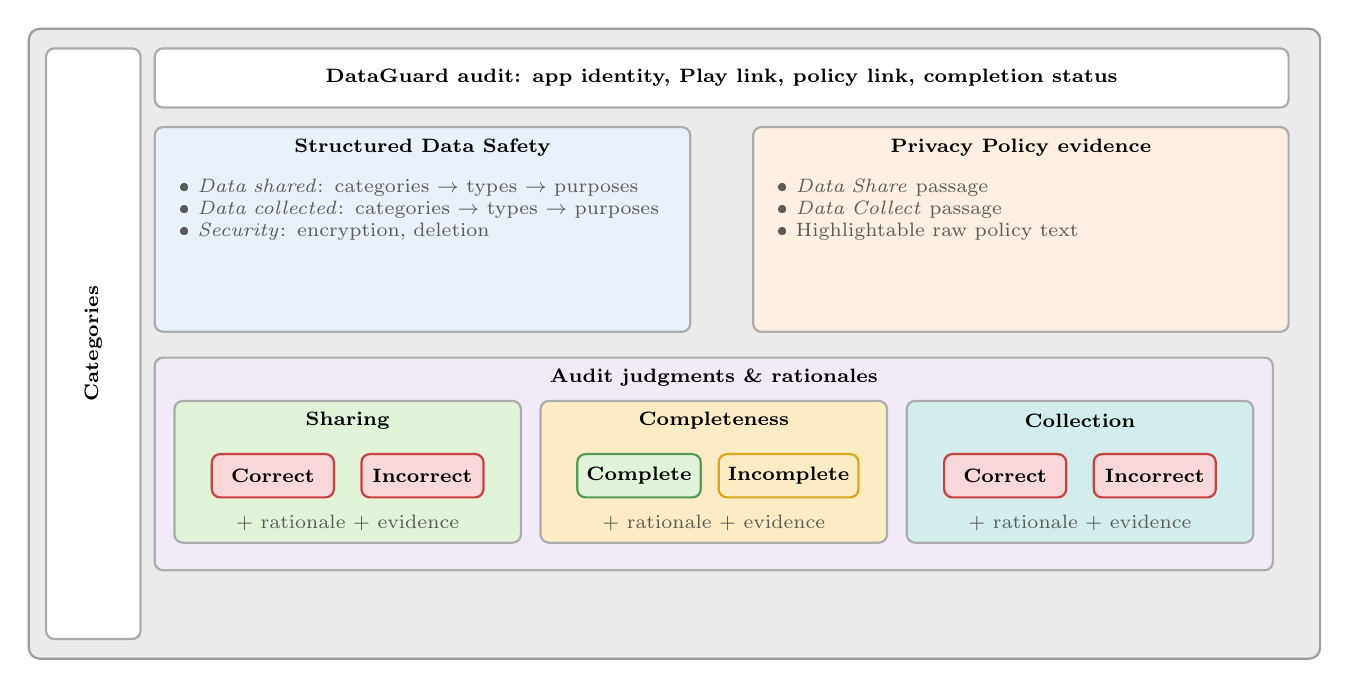
\begin{tikzpicture}[
  every node/.style={font=\small},
  win/.style={draw=dgGrey!60,thick,rounded corners=4pt,fill=dgGreyL},
  pane/.style={draw=dgGrey!50,thick,rounded corners=3pt,fill=white},
  caplbl/.style={font=\scriptsize\bfseries},
  hint/.style={font=\scriptsize,text=dgGrey},
  btn/.style={draw=dgRed,fill=dgRedL,thick,rounded corners=3pt,
              minimum height=0.55cm,minimum width=1.55cm,
              font=\scriptsize\bfseries}
]
\node[win,minimum width=16.4cm,minimum height=8.0cm] (W) at (0,0) {};

% sidebar
\node[pane,minimum width=1.2cm,minimum height=7.5cm,anchor=west]
   at ($(W.west)+(0.22,0)$) (side) {};
\node[caplbl,rotate=90] at (side.center) {Categories};

% header
\node[pane,minimum width=14.4cm,minimum height=0.75cm,anchor=north west]
   at ($(W.north west)+(1.6,-0.25)$) (head) {};
\node[caplbl] at (head.center)
   {\dataguard{} audit: app identity, Play link, policy link, completion status};

% data safety panel
\node[pane,fill=dgBlueL!60,minimum width=6.8cm,minimum height=2.6cm,
      anchor=north west]
   at ($(head.south west)+(0,-0.22)$) (DS) {};
\node[caplbl] at ($(DS.north)+(0,-0.27)$) {Structured Data Safety};
\node[hint,align=left,anchor=north west,text width=6.4cm]
   at ($(DS.north west)+(0.2,-0.55)$)
   {\textbullet\ \emph{Data shared}: categories $\rightarrow$ types $\rightarrow$ purposes\\
    \textbullet\ \emph{Data collected}: categories $\rightarrow$ types $\rightarrow$ purposes\\
    \textbullet\ \emph{Security}: encryption, deletion};

% policy panel
\node[pane,fill=dgOrangeL!60,minimum width=6.8cm,minimum height=2.6cm,
      anchor=north east]
   at ($(head.south east)+(0,-0.22)$) (PP) {};
\node[caplbl] at ($(PP.north)+(0,-0.27)$) {Privacy Policy evidence};
\node[hint,align=left,anchor=north west,text width=6.4cm]
   at ($(PP.north west)+(0.2,-0.55)$)
   {\textbullet\ \emph{Data Share} passage\\
    \textbullet\ \emph{Data Collect} passage\\
    \textbullet\ Highlightable raw policy text};

% judgments
\node[pane,fill=dgPurpleL!60,minimum width=14.2cm,minimum height=2.7cm,
      anchor=north west]
   at ($(DS.south west)+(0,-0.30)$) (J) {};
\node[caplbl] at ($(J.north)+(0,-0.27)$) {Audit judgments \& rationales};
% sharing block
\node[pane,minimum width=4.4cm,minimum height=1.8cm,anchor=north west,
      fill=dgGreenL]
   at ($(J.north west)+(0.25,-0.55)$) (Js) {};
\node[caplbl] at ($(Js.north)+(0,-0.27)$) {Sharing};
\node[btn] at ($(Js.center)+(-0.95,-0.05)$) {Correct};
\node[btn] at ($(Js.center)+( 0.95,-0.05)$) {Incorrect};
\node[hint] at ($(Js.south)+(0,0.27)$) {+ rationale + evidence};

\node[pane,minimum width=4.4cm,minimum height=1.8cm,anchor=north,
      fill=dgGoldL]
   at ($(J.north)+(0,-0.55)$) (Jc) {};
\node[caplbl] at ($(Jc.north)+(0,-0.27)$) {Completeness};
\node[btn,fill=dgGreenL,draw=dgGreen] at ($(Jc.center)+(-0.95,-0.05)$) {Complete};
\node[btn,fill=dgGoldL,draw=dgGold]  at ($(Jc.center)+( 0.95,-0.05)$) {Incomplete};
\node[hint] at ($(Jc.south)+(0,0.27)$) {+ rationale + evidence};

\node[pane,minimum width=4.4cm,minimum height=1.8cm,anchor=north east,
      fill=dgTealL]
   at ($(J.north east)+(-0.25,-0.55)$) (Jx) {};
\node[caplbl] at ($(Jx.north)+(0,-0.27)$) {Collection};
\node[btn] at ($(Jx.center)+(-0.95,-0.05)$) {Correct};
\node[btn] at ($(Jx.center)+( 0.95,-0.05)$) {Incorrect};
\node[hint] at ($(Jx.south)+(0,0.27)$) {+ rationale + evidence};
\end{tikzpicture}
\caption{Schematic of the \dataguard{} audit interface. The core
interaction is a side-by-side comparison between a structured Data Safety
panel and an extracted privacy-policy panel, followed by four categorical
judgments grouped into a Sharing, Completeness and Collection cluster,
each with a rationale and an evidence-paste box.}
\label{fig:interface}
\end{figure*}

\subsubsection{Annotation workflow}
\label{subsec:workflow}
Figure~\ref{fig:workflow} shows the annotation workflow. Annotators
first select a category and an app, then inspect the Data Safety and
Privacy Policy evidence side by side. For sharing and collection
separately, they judge correctness and completeness and record relevant
evidence or rationale. \dataguard{} stores each record with annotator
ID, time on task, and a unique evidence pointer. We use these records in
three ways: as label-row judgments for estimating potential auditability
problems (Studies~1--2), as paired labels for inter-annotator agreement
(Study~3), and as free-text rationales for analysing recurring sources
of audit difficulty (Study~4).

% --- Figure: workflow
\begin{figure}[t]
\centering
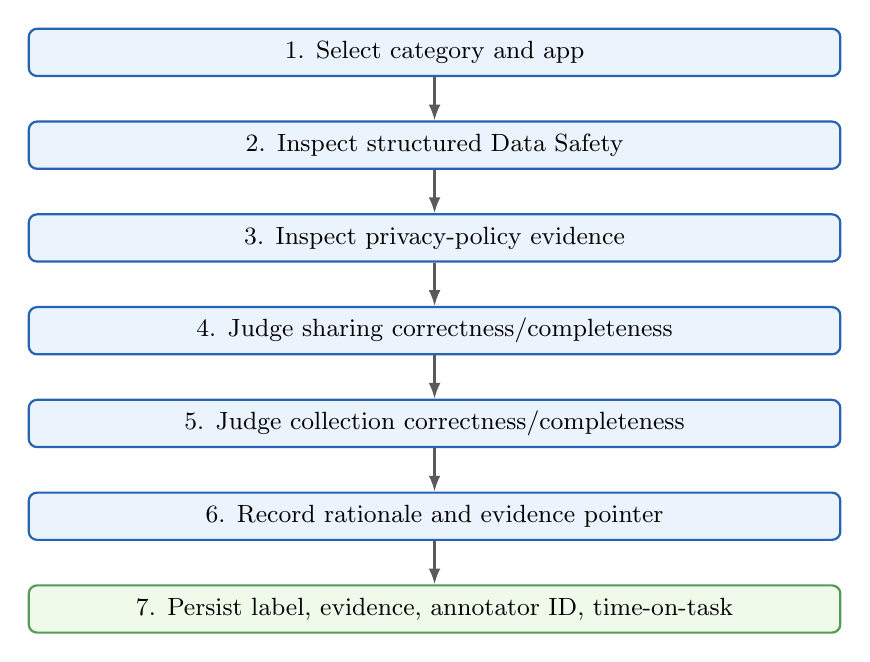
\begin{tikzpicture}[
  >={Latex[length=2.0mm]},
  node distance=0.55cm,
  wfstep/.style={draw=dgBlue,fill=dgBlueXL,rounded corners=3pt,thick,
               align=center,minimum width=0.85\columnwidth,minimum height=0.6cm,
               font=\small},
]
\node[wfstep] (s1) {1. Select category and app};
\node[wfstep,below=of s1] (s2) {2. Inspect structured Data Safety};
\node[wfstep,below=of s2] (s3) {3. Inspect privacy-policy evidence};
\node[wfstep,below=of s3] (s4) {4. Judge sharing correctness/completeness};
\node[wfstep,below=of s4] (s5) {5. Judge collection correctness/completeness};
\node[wfstep,below=of s5] (s6) {6. Record rationale and evidence pointer};
\node[wfstep,below=of s6,fill=dgGreenXL,draw=dgGreen] (s7)
   {7. Persist label, evidence, annotator ID, time-on-task};
\draw[->,thick,dgGrey] (s1) -- (s2);
\draw[->,thick,dgGrey] (s2) -- (s3);
\draw[->,thick,dgGrey] (s3) -- (s4);
\draw[->,thick,dgGrey] (s4) -- (s5);
\draw[->,thick,dgGrey] (s5) -- (s6);
\draw[->,thick,dgGrey] (s6) -- (s7);
\end{tikzpicture}
\caption{Annotation workflow used to collect human audit judgments in
\dataguard{}.}
\label{fig:workflow}
\end{figure}

\subsubsection{Why \dataguard{} is a research instrument, not a tool claim}
\label{subsec:rinstr}
We treat \dataguard{} as a probe that lets us observe the audit task
itself. We do \emph{not} claim that the interface improves end-user
accuracy or trust---those are system-performance claims that require a
controlled between-subjects study with end users, which we sketch in
Section~\ref{sec:future}. The justification for the present design is
that it makes visible the four artefacts that an automated pipeline would
otherwise discard: \emph{which} judgments human reviewers reach,
\emph{where} they disagree, \emph{which} policy fragments they pasted as
evidence, and \emph{why} (in their own words) the case was difficult.

% =====================================================================
\subsection{Data assets, annotators, and study design}
\label{sec:data}
% =====================================================================
\subsubsection{Data assets}
We use three nested data assets (Table~\ref{tab:assets}).
The crawled inventory contains $14{,}459$ Android package identifiers; the
metadata layer contains $12{,}876$ Play records; the structured
Data~Safety corpus contains $3{,}600$ scraped records of which $3{,}576$
parse cleanly. The audit workbook restricts to $2{,}400$ apps balanced as
$200$ per category and is the unit of annotation.

\begin{table}[t]
\centering
\small
\caption{Data assets, in order of nesting. Each layer is a subset of the
one above.}
\label{tab:assets}
\begin{tabular}{lrl}
\toprule
Asset & Size & Use \\
\midrule
Crawled package IDs        & $14{,}459$ & Sampling frame \\
Play metadata records       & $12{,}876$ & App context \\
Scraped Data Safety records & $3{,}600$  & Disclosure landscape \\
Parseable subset            & $3{,}576$  & Study~1 \\
Audit workbook              & $2{,}400$  & Audit task set \\
Audit judgments collected   & $1{,}506$  & Studies~2--4 \\
Unique apps audited         & $1{,}214$  & App-level results \\
Apps with $\geq 2$ annotators & $\sim286$ & Study~3 \\
Rationales captured         & $1{,}441$  & Study~4 \\
\bottomrule
\end{tabular}
\end{table}

\subsubsection{Annotators}
Seven annotators produced the audit corpus. The account ledger records
one PhD-level computer-science annotator (background in information
assurance), five senior software-engineering students (with declared
interests in AI and .NET), and one further student in AI. Annotators
were trained on a fixed protocol that defined \emph{Correct} as ``the
Data Safety claim is supported by, or consistent with, the policy
passage'' and \emph{Incorrect} as ``the policy contradicts, omits or
extends the claim in a substantive way''. Annotators were not lay
end-users; the design intent is to use trained reviewers as a proxy for
a regulator or motivated power user, and to isolate the difficulty of the
audit task itself from the additional difficulty of policy comprehension
by lay users. This framing matters for interpretation: our defect rates
are a \emph{floor}, not a typical end-user experience.

\subsubsection{Annotation coverage and quality checks}
Before interpreting substantive results, we assess whether the current
data are sufficiently complete for each claim. The crawler and parser
provide a strong basis for Study~1: in the canonical privacy-policy
output, $3{,}516$ of $3{,}599$ app records contain non-empty raw
policy text without an extraction error marker ($97.7\%$); $83$ records
are empty or error-like ($2.3\%$). For the Data Safety corpus, $3{,}576$
of $3{,}600$ records are parseable ($99.3\%$). In the annotation
workbook, $2{,}398$ of $2{,}400$ records have non-empty privacy-policy
content ($99.9\%$).

Annotation coverage varies across categories
(Table~\ref{tab:coverage}). Two categories (Art \& Design, Tools) have
complete coverage; four categories (Business, Communication, Lifestyle,
Social) are roughly half-covered; Personalization and Productivity have
no labels in the workbook used for this paper; Photography has only $27$
labelled apps. We therefore treat per-category human-label conclusions
as exploratory and explicitly flag Photography as low-coverage. Across
the full label set, $88.0\%$ of records contain a sharing-correctness
judgment, $96.0\%$ contain a collection-correctness judgment, $79.3\%$ a
sharing-completeness judgment, and $88.0\%$ a collection-completeness
judgment; $67.9\%$ contain all four. Crucially, $95.7\%$ contain at least
one non-empty evidence or rationale field, so the rationale signal is
much denser than any single categorical label
(Figure~\ref{fig:completeness}).

\begin{table}[t]
\centering\small
\caption{Human annotation coverage by app category in the audit workbook.
Coverage is computed over $200$ app records per category.}
\label{tab:coverage}
\begin{tabular}{lrrrr}
\toprule
Category & App records & Unique labelled & Label records & Coverage \\
\midrule
Art \& Design     & 200 & 200 & 216 & 100.0\% \\
Beauty            & 200 & 140 & 216 & 70.0\% \\
Books \& Ref.     & 200 & 145 & 145 & 72.5\% \\
Business          & 200 & 100 & 101 & 50.0\% \\
Communication     & 200 & 100 & 100 & 50.0\% \\
Lifestyle         & 200 & 101 & 103 & 50.5\% \\
Personalization   & 200 & 0   & 0   & 0.0\%  \\
Photography       & 200 & 27  & 27  & 13.5\% \\
Productivity      & 200 & 0   & 0   & 0.0\%  \\
Shopping          & 200 & 101 & 202 & 50.5\% \\
Social            & 200 & 100 & 136 & 50.0\% \\
Tools             & 200 & 200 & 260 & 100.0\% \\
\bottomrule
\end{tabular}
\end{table}

% --- Figure: completeness
\begin{figure}[t]
\centering
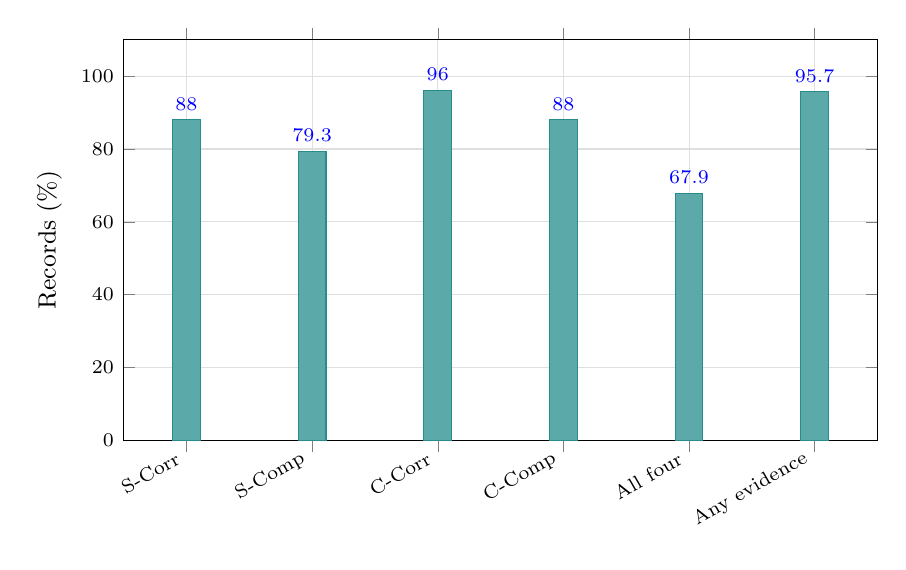
\begin{tikzpicture}
\begin{axis}[
  width=0.92\columnwidth,height=0.55\columnwidth,
  ybar,bar width=10pt,
  ymin=0,ymax=110,
  ylabel={Records (\%)},
  symbolic x coords={SCorr,SComp,CCorr,CComp,All4,Evid},
  xtick=data,
  xticklabels={S-Corr,S-Comp,C-Corr,C-Comp,All four,Any evidence},
  x tick label style={rotate=30,anchor=east,font=\scriptsize},
  nodes near coords,nodes near coords style={font=\scriptsize},
  grid=both,major grid style={draw=gray!25},
  tick label style={font=\scriptsize},label style={font=\small}
]
\addplot+[fill=dgTeal!75,draw=dgTeal] coordinates {
  (SCorr,88.0)(SComp,79.3)(CCorr,96.0)
  (CComp,88.0)(All4,67.9)(Evid,95.7)};
\end{axis}
\end{tikzpicture}
\caption{Completeness of the human audit records. Rationale or evidence
fields are non-empty far more often than any single categorical label
($95.7\%$ vs.\ $67.9\%$).}
\label{fig:completeness}
\end{figure}

\subsubsection{Research questions}
We organise the analysis into four studies.
\begin{description}[leftmargin=*,nosep,topsep=2pt]
\item[RQ1.]
What do Android apps actually declare in the Data Safety section, and
how does the disclosure landscape vary by category?
(\S\ref{sec:study1})
\item[RQ2.]
How often, and in which directions, do trained annotators flag Data
Safety disclosures as incorrect or incomplete when shown policy
evidence? (\S\ref{sec:study2})
\item[RQ3.]
Where do annotators disagree, and what does the agreement pattern
reveal about interpretive ambiguity? (\S\ref{sec:study3})
\item[RQ4.]
What recurring themes do annotator rationales surface, and how do those
themes map to interface requirements? (\S\ref{sec:study4})
\end{description}

\subsubsection{Study overview}
Figure~\ref{fig:study-flow} positions the four studies. Each study consumes
a sub-asset and produces evidence that feeds the design implications.

% --- Figure: study overview
\begin{figure*}[t]
\centering
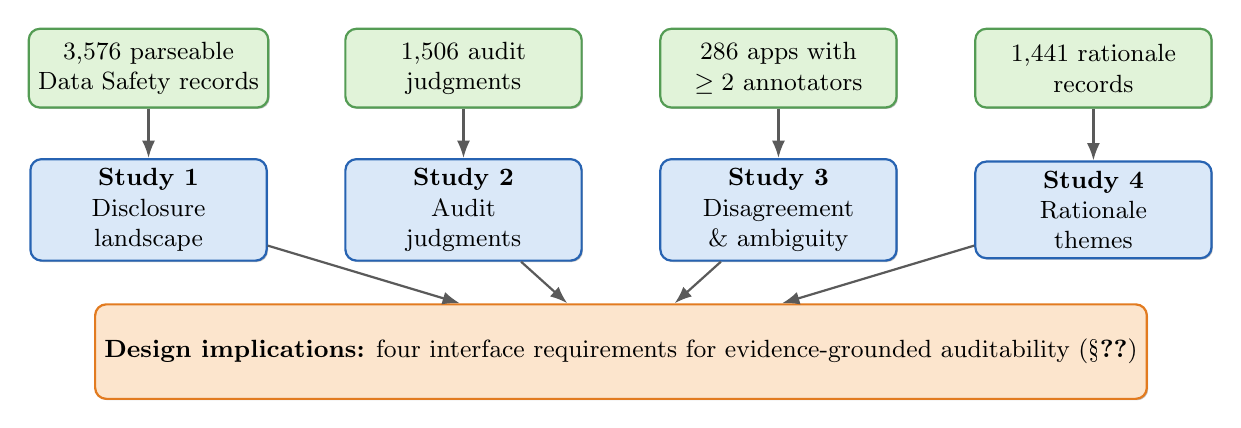
\begin{tikzpicture}[
  >={Latex[length=2.2mm]},
  every node/.style={font=\small},
  data/.style ={draw=dgGreen,fill=dgGreenL,thick,rounded corners=4pt,
                minimum width=3.0cm,minimum height=1.0cm,align=center,
                drop shadow={shadow xshift=0.5pt,shadow yshift=-0.5pt}},
  study/.style={draw=dgBlue,fill=dgBlueL,thick,rounded corners=4pt,
                minimum width=3.0cm,minimum height=1.2cm,align=center,
                drop shadow={shadow xshift=0.5pt,shadow yshift=-0.5pt}},
  design/.style={draw=dgOrange,fill=dgOrangeL,thick,rounded corners=4pt,
                 minimum width=11.6cm,minimum height=1.2cm,align=center,
                 drop shadow={shadow xshift=0.5pt,shadow yshift=-0.5pt}}
]
\node[data] (d1) at (0,0)   {$3{,}576$ parseable\\Data Safety records};
\node[data] (d2) at (4,0)   {$1{,}506$ audit\\judgments};
\node[data] (d3) at (8,0)   {$286$ apps with\\$\geq 2$ annotators};
\node[data] (d4) at (12,0)  {$1{,}441$ rationale\\records};

\node[study] (s1) at (0,-1.8)  {\textbf{Study 1}\\Disclosure\\landscape};
\node[study] (s2) at (4,-1.8)  {\textbf{Study 2}\\Audit\\judgments};
\node[study] (s3) at (8,-1.8)  {\textbf{Study 3}\\Disagreement\\$\&$ ambiguity};
\node[study] (s4) at (12,-1.8) {\textbf{Study 4}\\Rationale\\themes};

\node[design] (D) at (6,-3.6)
   {\textbf{Design implications:} four interface requirements for
    evidence-grounded auditability (\S\ref{sec:design})};

\foreach \i/\j in {d1/s1,d2/s2,d3/s3,d4/s4}
  \draw[->,thick,dgGrey] (\i) -- (\j);
\foreach \k in {s1,s2,s3,s4}
  \draw[->,thick,dgGrey] (\k) -- (D);
\end{tikzpicture}
\caption{Study overview. Each study consumes a slice of the corpus and
feeds the design implications in Section~\ref{sec:design}.}
\label{fig:study-flow}
\end{figure*}

\subsubsection{Metrics and statistical reporting}
For Study~1 we report the proportion of apps that declare at least one
shared data category, at least one collected data category, and no
shared or collected data, together with at least one security practice;
we also report Wilson $95\%$ confidence intervals on each proportion and
a category-level $\chi^{2}$ test with Cramer's $V$ as the effect size.
For Study~2 we report label-row proportions for each of the four
judgment axes, conditioning on non-empty rows, with Wilson $95\%$ CIs;
we also report an app-level robustness check using majority outcomes,
to ensure that label-row results are not driven by repeatedly-labelled
apps. For Study~3 we report Cohen's $\kappa$
\citep{cohen1960coefficient,landis1977measurement}
both with blank labels retained and on non-blank pairs only. For Study~4
we report lexical-scoping rates over rationale records, frame them as
\emph{candidate} codes for thematic analysis~\citep{braun2006using}, and
discuss why and how a full manual thematic-coding pass would extend the
present results.

% =====================================================================
% =====================================================================
\section{Empirical Findings}
\label{sec:findings}
% =====================================================================
\subsection{Study 1: Disclosure landscape}
\label{sec:study1}
% =====================================================================
\paragraph{Goal.} Characterise what the Data Safety section actually
claims across $3{,}576$ parseable Android-app records in $12$ Google-Play
categories.

\paragraph{Headline result.}
Across the parseable corpus, $39.7\%$ of apps declared at least one
shared data category (Wilson $95\%$~CI $38.1\text{--}41.3$), $45.3\%$
declared at least one collected data category ($43.7\text{--}46.9$),
and $39.5\%$ declared neither---the so-called \emph{empty} Data Safety
profile ($37.9\text{--}41.1$). Security practices were declared by
$80.9\%$ of records ($79.6\text{--}82.1$), but the typical security
practice was a generic \texttt{Data is encrypted in transit} entry. This
combination---broad security claims layered on top of empty data
claims---is itself an audit risk and motivates Study~2.

\paragraph{Category-level variation.}
Figure~\ref{fig:cat-disclosures} plots three indicators per category:
\emph{any-shared}, \emph{any-collected}, and \emph{no-data}. Shopping
apps declared collection most often ($79.0\%$); Beauty apps declared
neither sharing nor collection in $56.1\%$ of records. A $12$-way
$\chi^{2}$ test rejects the null that disclosure rates are uniform
across categories for all three indicators: \emph{any-shared}
$\chi^{2}(11)=99.63$, $p<.001$, $V=.167$; \emph{any-collected}
$\chi^{2}(11)=282.92$, $p<.001$, $V=.281$; \emph{no-data}
$\chi^{2}(11)=150.82$, $p<.001$, $V=.205$. A fourth test on
security-practice presence is also significant
($\chi^{2}(11)=89.34$, $p<.001$, $V=.158$). Auditability is therefore
\emph{not} a uniformly distributed problem; it concentrates in
categories whose policies are most likely to mention third-party SDKs
but whose labels are most likely to leave fields blank.

% --- Figure: category disclosures
\begin{figure*}[t]
\centering
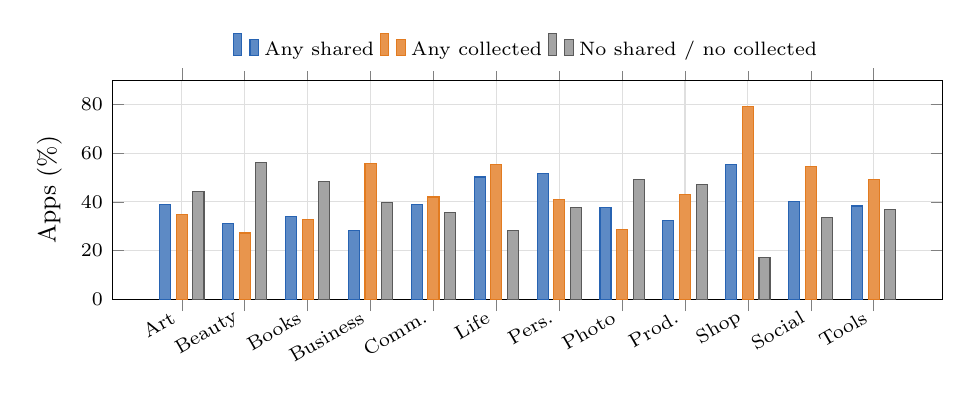
\begin{tikzpicture}
\begin{axis}[
  width=\textwidth,height=0.36\textwidth,
  ybar,bar width=4pt,
  ymin=0,ymax=90,
  ylabel={Apps (\%)},
  symbolic x coords={Art,Beauty,Books,Business,Comm,Life,Pers,Photo,Prod,Shop,Social,Tools},
  xtick=data,
  xticklabels={Art,Beauty,Books,Business,Comm.,Life,Pers.,Photo,Prod.,Shop,Social,Tools},
  x tick label style={rotate=30,anchor=east,font=\scriptsize},
  legend style={at={(0.5,1.04)},anchor=south,legend columns=3,
                draw=none,font=\scriptsize},
  grid=both,major grid style={draw=gray!25},minor grid style={draw=gray!10},
  tick label style={font=\scriptsize},label style={font=\small}
]
\addplot+[fill=dgBlue!75,draw=dgBlue]   coordinates {
  (Art,38.9)(Beauty,31.0)(Books,34.0)(Business,28.2)(Comm,39.0)
  (Life,50.2)(Pers,51.5)(Photo,37.5)(Prod,32.2)(Shop,55.3)
  (Social,40.1)(Tools,38.3)};
\addplot+[fill=dgOrange!80,draw=dgOrange] coordinates {
  (Art,34.8)(Beauty,27.2)(Books,32.7)(Business,55.7)(Comm,42.0)
  (Life,55.2)(Pers,40.8)(Photo,28.8)(Prod,43.0)(Shop,79.0)
  (Social,54.5)(Tools,49.3)};
\addplot+[fill=dgGrey!55,draw=dgGrey]   coordinates {
  (Art,44.4)(Beauty,56.1)(Books,48.5)(Business,39.6)(Comm,35.7)
  (Life,28.4)(Pers,37.8)(Photo,49.2)(Prod,47.3)(Shop,17.3)
  (Social,33.4)(Tools,37.0)};
\legend{Any shared,Any collected,No shared / no collected}
\end{axis}
\end{tikzpicture}
\caption{Data Safety disclosure patterns by Google-Play category
($n=3{,}576$ parseable records). Sharing and collection are not mutually
exclusive. All three category-level distributions differ from uniform
at $p<.001$.}
\label{fig:cat-disclosures}
\end{figure*}

\paragraph{Security-practice claims as a separate signal.}
We treat security-practice declarations as a third indicator alongside
sharing and collection because they appear in $80.9\%$ of records
and---per the $\chi^{2}$ test above---also vary significantly by
category. The bulk of those declarations are a single boilerplate
entry (\texttt{Data is encrypted in transit}), often with no
corresponding policy passage describing what is encrypted, with which
algorithm, or for which data subjects. From an auditability standpoint
this is a degenerate signal: it is highly readable, highly prevalent,
and provides essentially nothing on which to make a Correct/Incorrect
judgment. We therefore exclude security from the audit-judgment axes in
Studies~2 and~3 but report it here to make the asymmetry visible: the
field with the highest declaration rate is also the field with the
lowest audit content.

\paragraph{Most frequent data categories.}
Table~\ref{tab:topcats} reports the most frequently \emph{shared} and
\emph{collected} data categories. Identifiers and analytics-style
fields dominate both sides: \emph{Device or other IDs}, \emph{App info
and performance}, \emph{App activity}, \emph{Location}, and
\emph{Personal info}. These are exactly the categories that policies
are most likely to mention in oblique terms (\emph{cookies},
\emph{anonymous device data}, \emph{service providers}), which sets up
the auditability problem.

\begin{table}[t]
\centering\small
\caption{Top Data Safety data categories in the parseable corpus.}
\label{tab:topcats}
\begin{tabular}{lrr}
\toprule
Data category & Shared & Collected \\
\midrule
Device or other IDs       & $1{,}120$ & $1{,}186$ \\
App info and performance  & $705$     & $1{,}008$ \\
App activity              & $685$     & $909$     \\
Location                  & $557$     & $595$     \\
Personal info             & $350$     & $892$     \\
Photos and videos         & $155$     & $357$     \\
Financial info            & $143$     & $292$     \\
Messages                  & $93$      & $244$     \\
Files and documents       & $57$      & $163$     \\
\bottomrule
\end{tabular}
\end{table}

\paragraph{Purposes.}
At the purpose level, the dominant justifications were
\emph{App functionality}, \emph{Analytics}, \emph{Advertising or
marketing}, \emph{Fraud prevention, security, and compliance}. These
purposes matter for auditability because privacy policies often
describe the same practices using non-taxonomic terms such as
\emph{cookies}, \emph{advertising partners}, \emph{analytics
providers}, or \emph{service providers}. The mismatch between
purpose-as-platform-category and purpose-as-policy-prose is, as the
rationale analysis in Section~\ref{sec:study4} will show, one of the
single most cited sources of audit difficulty.

\paragraph{Implication for auditability.}
Study~1 establishes that the structured-disclosure channel itself is
already heterogeneous, category-skewed, and dominated by identifier-style
data. A trained reviewer arriving at this corpus is therefore already
working under a worst-case distribution of audit difficulty: many empty
labels, many identifier-only labels, and many security-only declarations
without enough scaffolding to map them onto a policy's narrative
description. Study~2 quantifies what happens next.

% =====================================================================
\subsection{Study 2: Human audit judgments}
\label{sec:study2}
% =====================================================================
\paragraph{Goal.} Quantify how trained annotators judge correctness and
completeness once they see structured Data Safety labels alongside the
extracted policy.

\subsubsection{Global outcomes}
Of $1{,}506$ judgments produced by seven annotators across $1{,}214$
apps, the \emph{sharing correctness} field was non-empty in $1{,}326$
cases; of those, $547$ ($41.3\%$, Wilson $95\%$~CI
$38.6\text{--}43.9$) were marked \emph{Incorrect}. The
\emph{sharing completeness} field was non-empty in $1{,}195$ cases;
$476$ ($39.8\%$, $37.1\text{--}42.6$) were \emph{Incomplete}.
\emph{Collection correctness} was non-empty in $1{,}446$ cases; $595$
($41.1\%$, $38.6\text{--}43.7$) were \emph{Incorrect}.
\emph{Collection completeness} was non-empty in $1{,}325$ cases; $591$
($44.6\%$, $41.9\text{--}47.3$) were \emph{Incomplete}
(Table~\ref{tab:global}). The app-level majority analysis returned
similar rates: $38.7\%$ of apps were majority-labelled as
sharing-incorrect, $40.9\%$ as sharing-incomplete, $39.9\%$ as
collection-incorrect, and $47.0\%$ as collection-incomplete. The
similarity between label-row and app-level summaries indicates that the
result is not driven solely by repeatedly-labelled apps. Aggregating
to the app level, $79.0\%$ of the $1{,}214$ audited apps received at
least one negative judgment.

\begin{table}[t]
\centering\small
\caption{Global audit outcomes. Rates are over non-empty judgments,
with Wilson $95\%$ CIs.}
\label{tab:global}
\begin{tabular}{lrrrr}
\toprule
Judgment & Negative label & Negative / non-empty & Rate & $95\%$ CI \\
\midrule
Sharing correctness     & Incorrect  & $547  / 1{,}326$ & $41.3\%$ & $38.6\text{--}43.9$ \\
Sharing completeness    & Incomplete & $476  / 1{,}195$ & $39.8\%$ & $37.1\text{--}42.6$ \\
Collection correctness  & Incorrect  & $595  / 1{,}446$ & $41.1\%$ & $38.6\text{--}43.7$ \\
Collection completeness & Incomplete & $591  / 1{,}325$ & $44.6\%$ & $41.9\text{--}47.3$ \\
\bottomrule
\end{tabular}
\end{table}

\subsubsection{Per-category average defect across the four axes}
For a per-category summary that we can defend directly from the audit
records, we compute the mean of the four directional rates plotted in
Figure~\ref{fig:cat-direction} (S-Incorrect, S-Incomplete, C-Incorrect,
C-Incomplete) for each labelled category. Figure~\ref{fig:defect-cat}
plots that mean. Average-axis defect rates range from $28.8\%$
(Shopping) to $54.7\%$ (Business), a $25.9$-point spread. The spread
is consistent with Study~1: categories with empty-label-heavy
disclosures (Business, Tools, Communication, Lifestyle) average more
negative judgments per app than categories with denser disclosures
(Shopping, Social).

% --- Figure: per-category average across the four axes
\begin{figure}[t]
\centering
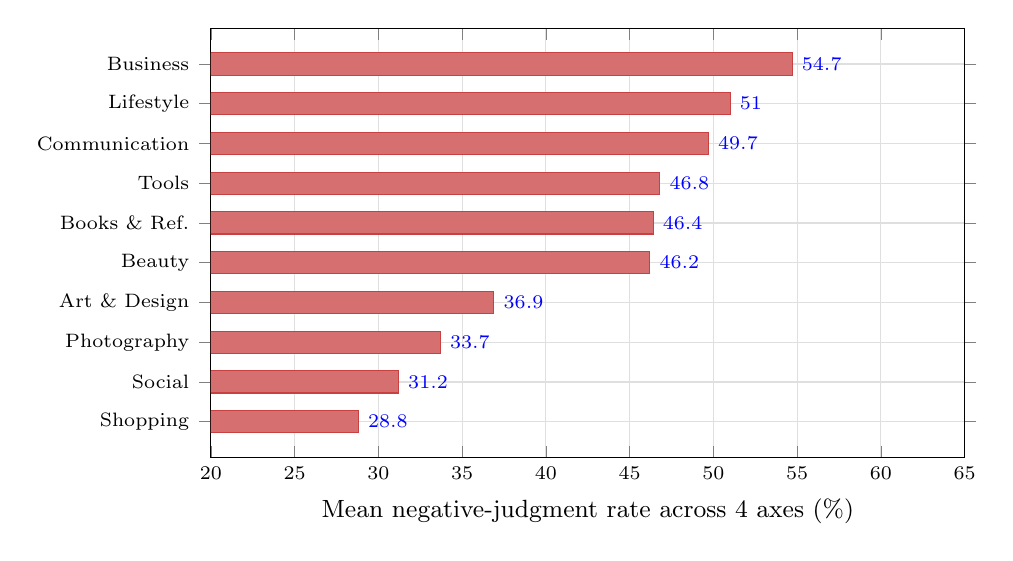
\begin{tikzpicture}
\begin{axis}[
  width=0.92\columnwidth,height=0.58\columnwidth,
  xbar,bar width=8pt,
  xmin=20,xmax=65,
  xlabel={Mean negative-judgment rate across 4 axes (\%)},
  symbolic y coords={Shop,Social,Photo,Art,Beauty,Books,Tools,Comm,Life,Business},
  ytick=data,
  yticklabels={Shopping,Social,Photography,Art \& Design,Beauty,
               Books \& Ref.,Tools,Communication,Lifestyle,Business},
  yticklabel style={font=\scriptsize},
  xticklabel style={font=\scriptsize},label style={font=\small},
  nodes near coords,
  nodes near coords style={font=\scriptsize},
  grid=major,major grid style={draw=gray!25}
]
\addplot+[fill=dgRed!75,draw=dgRed] coordinates {
  (28.8,Shop)(31.2,Social)(33.7,Photo)(36.9,Art)(46.2,Beauty)
  (46.4,Books)(46.8,Tools)(49.7,Comm)(51.0,Life)(54.7,Business)};
\end{axis}
\end{tikzpicture}
\caption{Per-category mean negative-judgment rate, averaged across
the four audit axes (sharing correctness/completeness and collection
correctness/completeness; data from Figure~\ref{fig:cat-direction}).
Categories with $<100$ labelled records (Photography) are reported but
should be interpreted cautiously.}
\label{fig:defect-cat}
\end{figure}

\subsubsection{Direction-of-error breakdown}
Figure~\ref{fig:cat-direction} shows the per-category breakdown for the
four judgment axes (categories with $\geq 100$ records). Business,
Beauty, Lifestyle, and Tools showed high \emph{Incorrect} rates for
both sharing and collection. Communication and Books \& Reference
showed especially high \emph{Incomplete} rates for collection
($61.8\%$ and $77.2\%$ respectively). Shopping, by contrast, had
comparatively low incomplete-collection ($13.1\%$), possibly because
shopping privacy policies tend to describe account, transaction and
service-provider data flows explicitly. This category-level shape
suggests that user-facing auditability support should not treat all
app categories as equivalent: different categories will need different
evidence prompts and different schema mappings.

% --- Figure: per-category 4-way breakdown
\begin{figure*}[t]
\centering
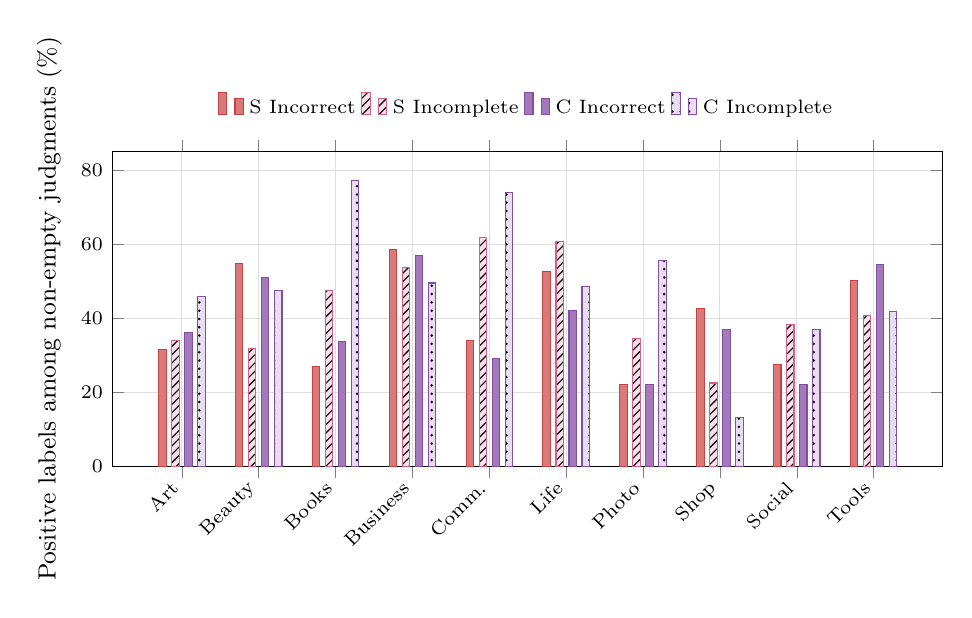
\begin{tikzpicture}
\begin{axis}[
  width=\textwidth,height=0.46\textwidth,
  ybar,bar width=2.7pt,
  ymin=0,ymax=85,
  ylabel={Positive labels among non-empty judgments (\%)},
  symbolic x coords={Art,Beauty,Books,Business,Comm,Life,Photo,Shop,Social,Tools},
  xtick=data,
  xticklabels={Art,Beauty,Books,Business,Comm.,Life,Photo,Shop,Social,Tools},
  x tick label style={rotate=45,anchor=east,font=\scriptsize},
  legend style={at={(0.5,1.07)},anchor=south,legend columns=4,draw=none,font=\scriptsize},
  grid=both,major grid style={draw=gray!25},minor grid style={draw=gray!10},
  tick label style={font=\scriptsize},label style={font=\small}
]
\addplot+[fill=dgRed!70,draw=dgRed] coordinates {
  (Art,31.6)(Beauty,54.7)(Books,27.0)(Business,58.6)(Comm,34.0)
  (Life,52.7)(Photo,22.2)(Shop,42.6)(Social,27.5)(Tools,50.2)};
\addplot+[fill=dgRoseL,draw=dgRose,postaction={pattern=north east lines}]
  coordinates {
  (Art,34.0)(Beauty,31.8)(Books,47.5)(Business,53.8)(Comm,61.8)
  (Life,60.8)(Photo,34.6)(Shop,22.5)(Social,38.2)(Tools,40.8)};
\addplot+[fill=dgPurple!75,draw=dgPurple] coordinates {
  (Art,36.2)(Beauty,51.0)(Books,33.8)(Business,57.0)(Comm,29.2)
  (Life,42.1)(Photo,22.2)(Shop,36.9)(Social,22.0)(Tools,54.5)};
\addplot+[fill=dgPurpleL,draw=dgPurple,postaction={pattern=dots}]
  coordinates {
  (Art,45.8)(Beauty,47.4)(Books,77.2)(Business,49.5)(Comm,73.9)
  (Life,48.5)(Photo,55.6)(Shop,13.1)(Social,36.9)(Tools,41.8)};
\legend{S Incorrect,S Incomplete,C Incorrect,C Incomplete}
\end{axis}
\end{tikzpicture}
\caption{Direction-of-error breakdown by app category. Personalization
and Productivity are omitted (no labels in the current workbook); the
Photography bar reflects only $27$ labelled apps and is plotted only for
visibility.}
\label{fig:cat-direction}
\end{figure*}

\subsubsection{No-data declarations are the worst audit case}
A central concern is apps whose Data Safety section declares
\emph{nothing}. Restricting to the audit rows whose Data Safety record
declared no shared data, $329$ of $703$ non-empty sharing judgments
were \emph{Incorrect}: $46.8\%$ (Wilson $95\%$~CI $43.1\text{--}50.5$).
Restricting to records declaring no collected data, $377$ of $633$
non-empty collection judgments were \emph{Incorrect}: $59.6\%$
($55.7\text{--}63.3$) (Figure~\ref{fig:no-data}). Empty labels do not
insulate apps from audit defects; they concentrate them. That
inversion---the easiest-to-read label is the hardest-to-audit
label---is the single sharpest result of this paper.

\begin{figure}[t]
\centering
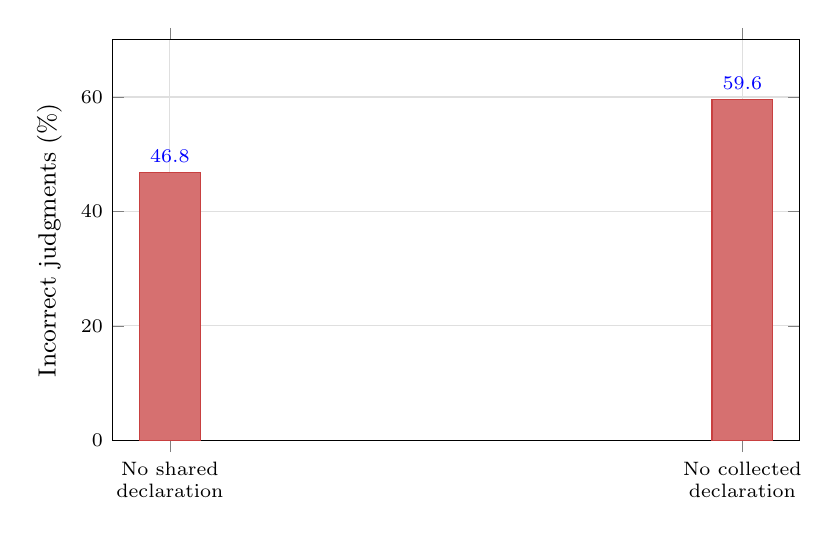
\begin{tikzpicture}
\begin{axis}[
  width=0.85\columnwidth,height=0.55\columnwidth,
  ybar,bar width=22pt,
  ymin=0,ymax=70,
  ylabel={Incorrect judgments (\%)},
  symbolic x coords={NoShared,NoCollected},
  xtick=data,
  xticklabels={No shared\\declaration,No collected\\declaration},
  x tick label style={align=center,font=\scriptsize},
  nodes near coords,
  nodes near coords style={font=\scriptsize\bfseries},
  grid=both,major grid style={draw=gray!25},minor grid style={draw=gray!10},
  tick label style={font=\scriptsize},label style={font=\small}
]
\addplot+[fill=dgRed!75,draw=dgRed] coordinates {
  (NoShared,46.8) (NoCollected,59.6)};
\end{axis}
\end{tikzpicture}
\caption{Incorrect-rate when the Data Safety section declares no
sharing (left) or no collection (right). Empty labels are the worst
case for audit, not the safest.}
\label{fig:no-data}
\end{figure}

\subsubsection{Coherent category-level signatures}
Beyond the per-axis split, Figure~\ref{fig:cat-direction} reveals
\emph{coherent} category-level signatures across the four axes.
Business, Beauty, Lifestyle, and Tools sit in the upper half of the
distribution on multiple axes simultaneously, while Shopping and
Social sit in the lower half on multiple axes. That coherence is
qualitatively inconsistent with a model in which negative judgments
are randomly distributed across axes; it is consistent with the view
that auditability is a property of the category-specific disclosure
\emph{regime}---the typical pairing of label content and policy prose
used in that category---rather than a per-app accident.

% =====================================================================
\subsection{Study 3: Disagreement and interpretive ambiguity}
\label{sec:study3}
% =====================================================================
\paragraph{Goal.} Determine whether the difficulty observed in Study~2
is intrinsic to the task or attributable to annotator variability.

\paragraph{Pairwise sample.}
We restrict to apps for which two distinct annotators produced an
audit record. The resulting double-annotated set contains $286$ apps
total, with non-blank sharing-correctness pairs in $237$ apps,
sharing-completeness in $181$, collection-correctness in $264$, and
collection-completeness in $226$. Raw agreement was modest: $34.3\%$ to
$52.4\%$ with blank labels retained and $50.3\%$ to $60.6\%$ on
non-blank pairs. On full agreement on the categorical label, we
observe $56.5\%$ for sharing-correctness and $56.1\%$ for
collection-correctness. We report Cohen's $\kappa$ both including blank
labels and conditioning on non-blank pairs (Table~\ref{tab:kappa}).

\begin{table}[t]
\centering\small
\caption{Inter-annotator agreement on double-annotated apps.
Interpretation follows~\citet{landis1977measurement}: $\kappa<0.20$ is
\emph{slight}.}
\label{tab:kappa}
\begin{tabular}{lrrrrrr}
\toprule
& \multicolumn{3}{c}{All pairs} & \multicolumn{3}{c}{Non-blank pairs}\\
\cmidrule(lr){2-4}\cmidrule(lr){5-7}
Judgment & $n$ & Agree & $\kappa$ & $n$ & Agree & $\kappa$\\
\midrule
Sharing correctness     & 286 & .507 & ~~.170 & 237 & .565 & ~~.140\\
Sharing completeness    & 286 & .343 & $-.090$ & 181 & .503 & $-.113$\\
Collection correctness  & 286 & .524 & ~~.101 & 264 & .561 & ~~.101\\
Collection completeness & 286 & .500 & ~~.114 & 226 & .606 & ~~.139\\
\bottomrule
\end{tabular}
\end{table}

\paragraph{What this tells us.}
None of the four $\kappa$ values clears the threshold for
slight-to-fair agreement, and the completeness axes are
indistinguishable from chance. That pattern is inconsistent with an
inattention story---the annotators were trained, used the same
interface, and looked at the same materials---and consistent with the
interpretive-ambiguity story: \emph{completeness} requires a reviewer
to decide what should have been said but was not, which is harder than
detecting an outright contradiction. Figure~\ref{fig:kappa} plots the
four values with the slight/fair guidance band
of~\citet{landis1977measurement} for reference.

% --- Figure: kappa
\begin{figure}[t]
\centering
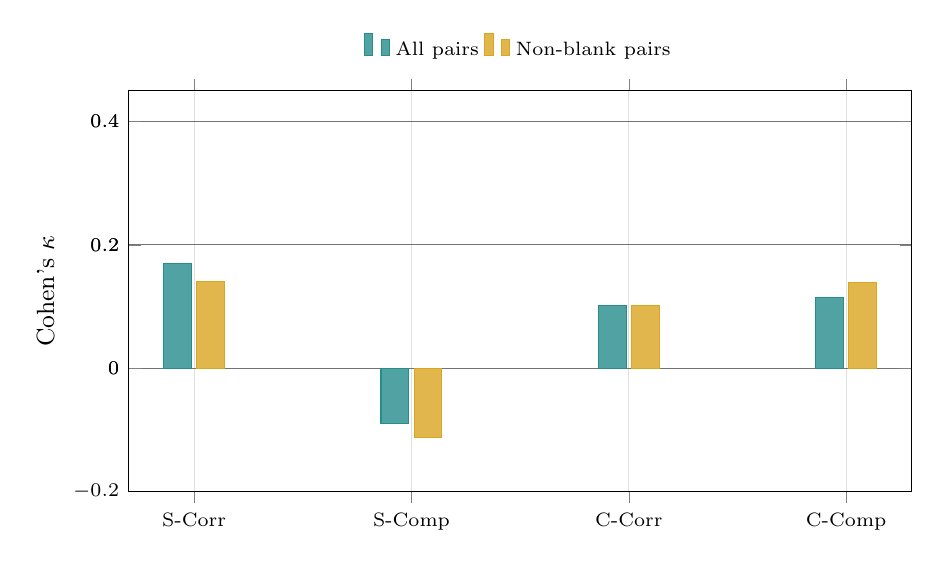
\begin{tikzpicture}
\begin{axis}[
  width=0.95\columnwidth,height=0.55\columnwidth,
  ybar,bar width=10pt,
  ymin=-0.20,ymax=0.45,
  ylabel={Cohen's $\kappa$},
  symbolic x coords={SCorr,SComp,CCorr,CComp},
  xtick=data,xticklabels={S-Corr,S-Comp,C-Corr,C-Comp},
  x tick label style={font=\scriptsize},label style={font=\small},
  legend style={at={(0.5,1.05)},anchor=south,legend columns=2,draw=none,
                font=\scriptsize},
  grid=both,major grid style={draw=gray!25},minor grid style={draw=gray!10},
  tick label style={font=\scriptsize},
  extra y ticks={0,0.20,0.40},
  extra y tick style={grid=major,major grid style={draw=black!55}}
]
\addplot+[fill=dgTeal!80,draw=dgTeal] coordinates {
  (SCorr,0.170)(SComp,-0.090)(CCorr,0.101)(CComp,0.114)};
\addplot+[fill=dgGold!80,draw=dgGold] coordinates {
  (SCorr,0.140)(SComp,-0.113)(CCorr,0.101)(CComp,0.139)};
\legend{All pairs,Non-blank pairs}
\end{axis}
\end{tikzpicture}
\caption{Cohen's $\kappa$ for the four audit judgments. The reference
grid line at $0.20$ is the \emph{slight}/\emph{fair} boundary
in~\citet{landis1977measurement}. All four values fall below
\emph{slight}.}
\label{fig:kappa}
\end{figure}

\paragraph{Per-axis interpretation.}
Aggregate $\kappa$ collapses two genuinely different mental
subroutines---detecting a contradiction (\emph{correctness}) and
deciding that something has been left out (\emph{completeness})---into
a single number. Reporting $\kappa$ separately by axis, as
Table~\ref{tab:kappa} does, makes the asymmetry visible: completeness
is consistently the harder axis. A category-level analysis would also
be informative; we leave a fully powered axis-by-category $\kappa$
analysis to the adjudication study described in \S\ref{sec:future}.

\paragraph{What disagreement looks like.}
Two kinds of disagreement dominated. The first was a
sharing/collection asymmetry: one annotator located a third-party
mention in the policy and judged sharing as \emph{Incorrect}, while
the other read the same mention as a description of the developer's
own data collection (not sharing). The second was an evidence-vs.-hedge
asymmetry: a policy line such as ``\emph{we may share information
with affiliates and service providers}'' was judged \emph{Incorrect}
by one annotator (the label omits sharing) and \emph{Correct} by
another (the policy never asserts that sharing actually occurs). Both
disagreement patterns are direct symptoms of the auditability gap, not
of annotator competence.

% =====================================================================
\subsection{Study 4: Rationale themes for design}
\label{sec:study4}
% =====================================================================
\paragraph{Goal.} Use the free-text rationale field to surface
\emph{why} the audit task is hard, and produce a candidate codebook
for a follow-on manual thematic analysis.

\paragraph{Lexical scoping.}
Of $1{,}506$ judgments, $1{,}441$ ($95.7\%$) contain at least one
non-empty rationale or evidence field. We performed a lexical scoping
pass over those rationales using seven indicator families (third-party,
generic-hedging, identifier-and-cookie, no-data-contradiction, location
ambiguity, security/deletion, and external responsibility). The
indicators are pre-coding: their role is to circumscribe themes for
manual coding in line with~\citet{braun2006using}, not to substitute
for it. Indicator rates are reported in Table~\ref{tab:themes} and
visualised in Figure~\ref{fig:themes}.

\begin{table}[t]
\centering\small
\caption{Candidate rationale themes (lexical scoping over
$1{,}441$ rationale records).}
\label{tab:themes}
\begin{tabular}{p{0.30\columnwidth}rp{0.55\columnwidth}}
\toprule
Theme & Rate & Why it makes audit hard\\
\midrule
Third-party ads / analytics  & $54.5\%$ & Policies cite SDKs, vendors,
   ``service providers'', or named platforms; mapping to Data Safety
   sharing categories is non-trivial.\\
Generic legal hedging        & $44.7\%$ & Phrases like ``may collect'',
   ``including but not limited to'' resist a binary correct/incorrect
   judgment.\\
Device identifiers \& cookies& $35.5\%$ & IP, advertising ID, MAC,
   SIM identifiers cross multiple Data Safety categories.\\
No-data contradiction        & $30.4\%$ & The Data Safety section
   declares nothing while the policy discusses ads, analytics or IDs.\\
Location ambiguity           & $12.3\%$ & Policies mention coarse or
   IP-derived location without a matching Location field.\\
Security / deletion          & $11.0\%$ & Generic encryption and
   retention claims are difficult to test against any concrete claim.\\
External responsibility      & $6.2\%$  & Policies push responsibility
   to linked sites or third parties, leaving label scope ambiguous.\\
\bottomrule
\end{tabular}
\end{table}

% --- Figure: themes (sized to text width)
\begin{figure}[t]
\centering
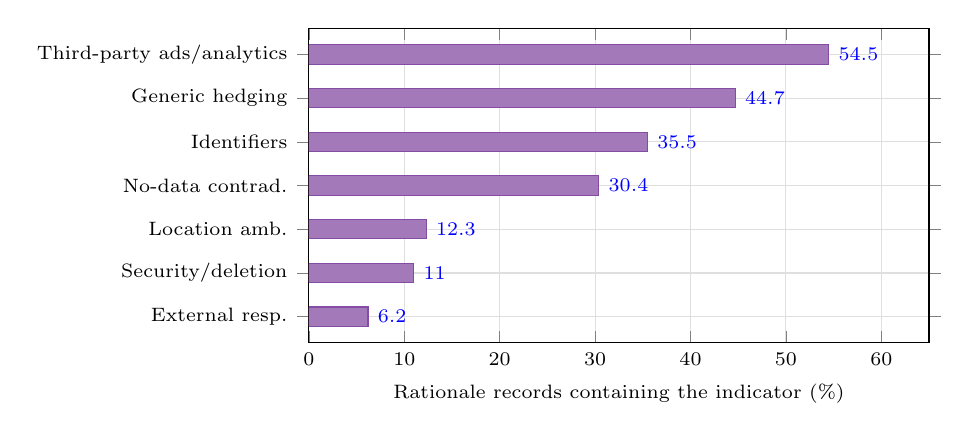
\begin{tikzpicture}
\begin{axis}[
  width=0.78\columnwidth,height=0.46\columnwidth,
  xbar,bar width=7pt,
  xmin=0,xmax=65,
  xlabel={Rationale records containing the indicator (\%)},
  symbolic y coords={External,Security,Location,NoData,IDs,Generic,Third},
  ytick=data,
  yticklabels={External resp.,Security/deletion,Location amb.,
               No-data contrad.,Identifiers,Generic hedging,
               Third-party ads/analytics},
  yticklabel style={font=\scriptsize},
  xticklabel style={font=\scriptsize},label style={font=\scriptsize},
  nodes near coords,
  nodes near coords style={font=\scriptsize},
  grid=major,major grid style={draw=gray!25},
  enlarge y limits=0.10
]
\addplot+[fill=dgPurple!75,draw=dgPurple] coordinates {
  (6.2,External)(11.0,Security)(12.3,Location)(30.4,NoData)
  (35.5,IDs)(44.7,Generic)(54.5,Third)};
\end{axis}
\end{tikzpicture}
\caption{Lexical-scoping rates for seven candidate rationale themes
($n=1{,}441$ rationale records).}
\label{fig:themes}
\end{figure}

\paragraph{Illustrative examples.}
For each theme, the rationale corpus contains many short, recurring
exemplars. \emph{Third-party}: ``Policy mentions Google AdMob and
Firebase but Data Safety lists no sharing.'' \emph{Generic hedging}:
``Policy uses `may share with affiliates'---we cannot tell whether
the app actually shares.'' \emph{Identifiers}: ``Policy mentions IP,
ad ID and device ID, but Data Safety only lists `Device or other
IDs', so we cannot tell which.'' \emph{No-data contradiction}:
``Data Safety: nothing. Policy: half a page on cookies and analytics.''
These are not edge cases; they are the modal rationale text.

\paragraph{Evidence-paste corpus as a secondary signal.}
Beyond the rationale free text, many records also contain a verbatim
\emph{evidence-paste} field: a policy passage that the annotator
considered decisive for the judgment. This corpus is a usable
training signal for an evidence-locator model
(see~\S\ref{sec:future}): every paste records a (structured-claim,
policy-span) pair against which an evidence-grounded policy QA
model~\citep{ravichander2019question,ahmad2021intent} can be evaluated.

\paragraph{Co-occurrence of themes (qualitative).}
The seven indicators are not mutually exclusive; many rationale
records cite more than one. Qualitatively, the most prominent pair is
\emph{third-party plus identifiers}: a policy that mentions advertising
IDs, cookies and analytics SDKs in a vendor-neutral way, leaving the
reviewer to decide whether the identifier is being collected, shared,
or both, and by whom. The second prominent pair is \emph{no-data plus
third-party}: an empty Data Safety label paired with a policy that
defers responsibility to third parties. Both pairs match cases that
the contextual-integrity tradition flags as hardest: the data flow is
intelligible at a high level but its actor graph is under-specified.
A formal co-occurrence analysis of the rationale corpus is part of
the manual thematic-coding step we outline in \S\ref{sec:future}.

\paragraph{From themes to design entry points.}
The four heaviest themes (Third-party, Generic hedging, Identifiers,
No-data) are the same four themes that the automated pipelines of
\citet{andow2019policylint} and \citet{andow2020policheck} identified
as hardest for their classifiers. We read this as a consistency
check: the points where automated analysis breaks down are also the
points where human annotators ask for help. This is exactly the
design opportunity that Section~\ref{sec:design} pursues.

% =====================================================================
\section{Design Implications}
\label{sec:design}
% =====================================================================
The four heaviest themes from Study~4 become four interface
requirements. We state each as a rule for designers of future
privacy-disclosure UIs, not as a feature of \dataguard{} itself.
Figure~\ref{fig:requirements} shows the four requirements as a
colour-coded ring around the human reviewer.

\paragraph{\dgrule{1} Evidence-first labels.}
Whenever the interface displays a structured Data Safety claim, the
underlying policy fragment used to derive that claim should be one
click away. Inspired by the evidence-grounded review style of
CLAUDETTE~\citep{lippi2019claudette} and the human-AI principles
of~\citet{amershi2019guidelines} and~\citet{cai2019hello}, the rule
inverts the current Play layout: rather than a label that hides its
source, the label \emph{is} a window onto its source.
Implementationally, every category, type and purpose displayed in a
label should resolve to a span of policy text (or to an explicit
``no supporting evidence'' state).

\paragraph{\dgrule{2} Ambiguity-aware review states.}
Study~3 shows that forcing every case into Correct/Incorrect or
Complete/Incomplete erases real ambiguity. The interface should permit
\emph{ambiguity} as a first-class state, with concrete sub-types
(\emph{insufficient evidence}, \emph{policy too generic},
\emph{taxonomy mismatch}, \emph{third-party responsibility unclear}).
These match the four heaviest rationale themes. The lower the agreed-on
verdict between annotators, the more important it is to provide a
non-binary control.

\paragraph{\dgrule{3} Taxonomy-mapping support.}
Many rationales mention policy terms (\emph{advertising ID},
\emph{IP address}, \emph{cookie}, \emph{service provider}) that do not
appear in the Data Safety schema. A small structured glossary that
maps such terms to candidate Data Safety categories and purposes turns
the cognitive mapping step into a UI affordance. The glossary is itself
a research artefact: it can be reused across studies, extended by
crowdsourced editing, and validated against the OPP-115
schema~\citep{wilson2016creation} or the intent slots
of~\citet{ahmad2021intent}.

\paragraph{\dgrule{4} Third-party flow visibility.}
The single heaviest theme is third-party sharing. Future label UIs
should visualise third-party recipients explicitly, distinguishing the
app developer, analytics SDKs, ad networks and linked sites, and
distinguishing collection from onward sharing. This requirement
intersects with the runtime ecosystem mapping of
\citet{razaghpanah2018apps} and the policy-level analysis of
\citet{andow2020policheck}: a usable label needs to surface the actor
graph that those papers reconstruct under the hood.

% --- Figure: requirements ring (text-width, single column)
\begin{figure}[t]
\centering
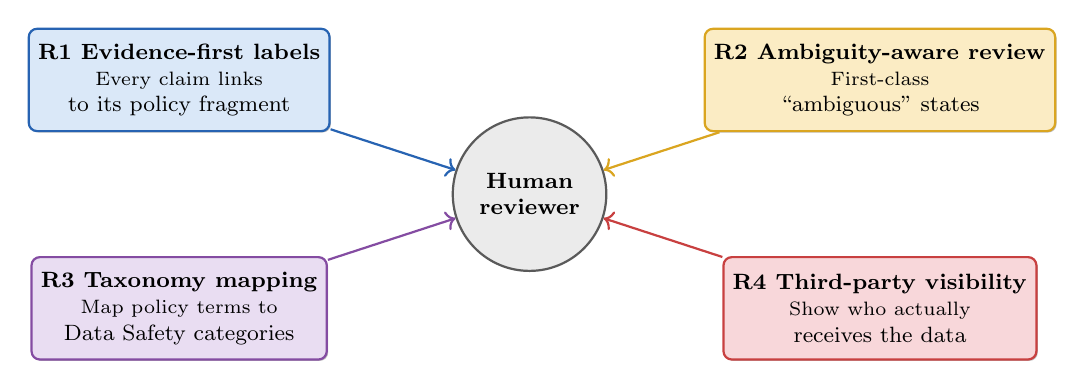
\begin{tikzpicture}[
  every node/.style={font=\footnotesize},
  hub/.style={draw=dgGrey,fill=dgGreyL,thick,circle,
              minimum size=1.95cm,align=center},
  req/.style={draw,thick,rounded corners=3pt,
              minimum width=3.55cm,minimum height=1.3cm,align=center,
              drop shadow={shadow xshift=0.5pt,shadow yshift=-0.5pt}}
]
\node[hub] (H) at (0,0) {\textbf{Human}\\\textbf{reviewer}};

\node[req,draw=dgBlue,  fill=dgBlueL]   (R1) at (-4.45, 1.45)
  {\textbf{R1 Evidence-first labels}\\\scriptsize Every claim links\\to its policy fragment};
\node[req,draw=dgGold,  fill=dgGoldL]   (R2) at ( 4.45, 1.45)
  {\textbf{R2 Ambiguity-aware review}\\\scriptsize First-class\\``ambiguous'' states};
\node[req,draw=dgPurple,fill=dgPurpleL] (R3) at (-4.45,-1.45)
  {\textbf{R3 Taxonomy mapping}\\\scriptsize Map policy terms to\\Data Safety categories};
\node[req,draw=dgRed,   fill=dgRedL]    (R4) at ( 4.45,-1.45)
  {\textbf{R4 Third-party visibility}\\\scriptsize Show who actually\\receives the data};

\draw[->,thick,dgBlue]   (R1) -- (H);
\draw[->,thick,dgGold]   (R2) -- (H);
\draw[->,thick,dgPurple] (R3) -- (H);
\draw[->,thick,dgRed]    (R4) -- (H);
\end{tikzpicture}
\caption{The four interface requirements wrap around the human
reviewer. Each requirement targets the heaviest theme in Study~4 and
addresses a failure mode observed in Studies~2 and~3.}
\label{fig:requirements}
\end{figure}

\paragraph{An evidence-first reframing of the label.}
Taken together, the four requirements imply a structural reframing
of the Data Safety label. In the current design the label is the
\emph{primary} surface and the policy is a hidden secondary surface
linked by a single hyperlink; the audit task is, at best, a
secondary affordance of that pairing. Under the four requirements, the
label becomes a \emph{view} onto an evidence-grounded data structure
whose primary content is the policy text, indexed and annotated by the
structured claims. The structural inversion has three consequences.
First, it makes the auditability gap measurable in the interface
itself: the share of a label's tokens whose evidence is missing or
ambiguous is now a UI-visible field. Second, it shifts the locus of
labour from the reader to the toolchain: rather than asking a human
to construct the label-evidence mapping in their head, the system
displays it, with explicit ``no evidence'' or ``ambiguous'' states
where appropriate. Third, it makes the label a contestable artefact:
a reader who disagrees with the highlighted evidence can record that
disagreement, which feeds back into a public-trust signal of the kind
that comparative-privacy interfaces have long aspired
to~\citep{tsai2011effect,kelley2010standardizing} but rarely
delivered.

\paragraph{Sketch of an evidence-first label UI.}
Concretely, an evidence-first Data Safety label would render each
structured claim as a chip carrying the claim text, the linked policy
span, and a short evidence-state indicator (\emph{supported},
\emph{contradicted}, \emph{ambiguous}, \emph{no evidence}). Hovering
or clicking a chip would expand its evidence panel. A category-level
summary chip would show the share of supported vs.\ unsupported
sub-claims, so that a reader could see at a glance whether the
\emph{label is auditable at all} before judging whether they trust
its content. Such a UI does not require AI assistance to operate;
it only requires that the platform commit to publishing labels paired
with the evidence spans that justify them. AI assistance, when
present, becomes a labour-saving accelerator for the platform-side
annotator, not a substitute for the evidence link itself.

\paragraph{Cross-walk: from finding to requirement.}
Table~\ref{tab:findings-to-req} cross-walks each finding to a
requirement and to a literature precedent. The intent is to show that
the four design rules do not float free of the data: each is fitted
to a specific pattern in the audit corpus and supported by an
established precedent in the HCI or accountability literature.

\begin{table*}[t]
\centering\small
\caption{Cross-walk from empirical finding to design requirement.}
\label{tab:findings-to-req}
\begin{tabular}{p{0.30\textwidth}p{0.18\textwidth}p{0.46\textwidth}}
\toprule
Empirical finding & Requirement & Precedent in the literature \\
\midrule
Defects pervasive ($79.0\%$), category-dependent and concentrated on
no-data labels (\S\ref{sec:study2})
& \dgrule{1} Evidence-first labels
& Evidence-grounded compliance review~\citep{lippi2019claudette};
  human-AI design~\citep{amershi2019guidelines,cai2019hello};
  XAI questioning practice~\citep{liao2020questioning}.
\\[2pt]
$\kappa<0.20$ across all four judgment axes, completeness worst
(\S\ref{sec:study3})
& \dgrule{2} Ambiguity-aware review states
& Vagueness theory in policy text~\citep{bhatia2016theory};
  OPP-115 inter-annotator results~\citep{wilson2016creation};
  contextual integrity as a property of legitimacy~\citep{nissenbaum2004privacy}.
\\[2pt]
Identifier / cookie / service-provider terminology drives $35.5\%$ of
rationales (\S\ref{sec:study4})
& \dgrule{3} Taxonomy-mapping support
& Intent slots for policy NLP~\citep{ahmad2021intent};
  PolicyLint negation logic~\citep{andow2019policylint};
  PrivacyFlash / MAPS taxonomy~\citep{zimmeck2019maps}.
\\[2pt]
Third-party SDK / analytics references in $54.5\%$ of rationales
(\S\ref{sec:study4})
& \dgrule{4} Third-party flow visibility
& Entity-sensitive flow analysis~\citep{andow2020policheck};
  global tracker ecosystem~\citep{razaghpanah2018apps,englehardt2016online};
  Lalaine Apple-label non-compliance~\citep{xiao2023lalaine}.
\\
\bottomrule
\end{tabular}
\end{table*}

% =====================================================================
\section{Discussion}
\label{sec:discussion}
% =====================================================================
\subsection{Auditability and its position in the HCI triangle}
\label{sec:disc-triangle}
We treat \emph{auditability} as the third leg of a triangle whose
first two legs are \emph{readability} and \emph{accuracy}. Readability
research asks whether a label is understood by a reader; accuracy
research asks whether the label matches the world; auditability asks
whether the \emph{link} between the label and its evidence is
traversable by a human. That property has been an implicit assumption
of label-based transparency since~\citet{kelley2009nutrition}; we
make it explicit and measurable. The framing sits naturally alongside
Nissenbaum's contextual-integrity account of
privacy~\citep{nissenbaum2004privacy}: contextual integrity asks
whether a data flow respects the norms of its origin context;
auditability asks whether a person can \emph{tell}, from the available
textual artefacts, that the flow does or does not respect those
norms. In that sense auditability is the epistemic precondition of
contextual integrity at the platform-disclosure level: a flow that
cannot be audited cannot be assigned a norm-respecting verdict at all.
The four audit failure modes in Section~\ref{sec:concept} map cleanly
onto contextual-integrity constructs: \textsc{Contradict} matches a
violated transmission norm, \textsc{Omit} matches a hidden context, and
\textsc{Ambig} matches under-determined contexts in which the available
evidence is insufficient to fix a norm.

It is worth being explicit about what \dataguard{} does and does not
let us claim. The instrument and the corpus reveal \emph{where}
privacy-label audit breaks down, \emph{which} policy fragments humans
treat as decisive, and \emph{which} kinds of ambiguity recur across
categories. They do not yet reveal whether any of the four design
requirements actually improves end-user accuracy, calibration, or
trust: that is a prospective-study claim that we sketch in
Section~\ref{sec:future}. The retrospective evidence is sufficient to
motivate the requirements; the prospective evidence is what would
license a stronger system-performance claim.

\subsection{No-data labels are the audit hot-spot, and disagreement is signal}
\label{sec:disc-nodata}
The most prevalent failure mode in our corpus is the empty label: a
Data Safety disclosure that declares neither sharing nor collection.
Such a label is the easiest to read---there is nothing to read---and
the hardest to audit, because any non-trivial policy will mention at
least \emph{some} data practice that conflicts with the empty claim.
We saw this in two forms: $39.5\%$ of parseable records were empty
(Section~\ref{sec:study1}), and $46.8$--$59.6\%$ of non-empty audit
judgments on those records were marked \emph{Incorrect}
(Section~\ref{sec:study2}). Treating no-data labels as the audit
hot-spot is a concrete implication of our results: operationally, a
platform could refuse to accept a no-data label without at least an
evidence pointer to the policy, because a policy that discusses
analytics SDKs cannot reasonably co-exist with a no-sharing claim.

The low $\kappa$ values in Section~\ref{sec:study3} would normally
suggest weak data quality. We read them as a substantive finding
instead. The same materials, presented through the same interface to
seven trained reviewers, produced systematically interpretive
disagreement, with completeness the hardest axis. This is consistent
with~\citet{bhatia2016theory}'s account of vagueness in privacy text
and with~\citet{wilson2016creation}'s OPP-115 observation that
fine-grained labels resist high-agreement annotation. Auditability
research therefore needs metrics that treat ambiguity as a measurable
property of the disclosure rather than as a residual of an annotation
pipeline.

\subsection{Reconciling with the automated mismatch literature, and the corpus as benchmark}
\label{sec:disc-reconcile}
Our $79.0\%$ app-level defect rate is, on its face, much higher than
the rates reported by automated pipelines: PolicyLint flagged
$14.2\%$ of $11{,}430$ Play policies as internally
contradictory~\citep{andow2019policylint}; PoliCheck flagged up to
$42.4\%$ of $13{,}796$ apps for incorrect or undisclosed sensitive
flows~\citep{andow2020policheck}. The numbers are not directly
comparable: automated pipelines fix a narrow classifier vocabulary
(typically person-identifying data flows on specific channels) and
optimise for high precision at the cost of recall; our human reviewers
were instructed to use the broader definition the platform itself
applies, including ambiguous cases and across all four judgment axes.
Both literatures nevertheless point in the same direction: under
\emph{any} reasonable operationalisation, a large fraction of Data
Safety disclosures are not unambiguously supported by the policy.
Our additional contribution is to show that what looks under the
automated lens like a narrow precision-tuned classifier problem is,
under the human lens, a much broader and more interpretive gap, with
completeness as the worst axis.

The audit corpus is therefore a useful benchmark for the next round
of evidence-grounded auditability assistance. Three benchmarking modes
are natural. \emph{Label-only mode}: given a structured Data Safety
claim, predict the four categorical judgments. \emph{Evidence-only
mode}: given the policy text, retrieve the span that a human reviewer
would paste as decisive evidence. \emph{Joint mode}: produce both the
categorical judgment and the supporting span, and measure them against
the human-paste corpus. The last mode is the most informative because
it captures design rule \dgrule{1} (evidence-first) at the evaluation
boundary: a model that predicts the right label for the wrong reason
is penalised. We argue that the appropriate metric pair is per-axis
balanced F1 for the categorical judgment and span-level overlap (IoU
or exact-match) against the human paste; reporting accuracy alone is
explicitly insufficient. We expect that current evidence-grounded
policy QA models~\citep{ravichander2019question} will be most accurate
on the two label-supported corners (\textsc{Ok},
\textsc{Contradict}) and least accurate on the two ambiguity corners
(\textsc{Omit}, \textsc{Ambig}), which is exactly the asymmetry that
motivates an \emph{ambiguity-aware} interface (\dgrule{2}).

\subsection{Threats to validity, regulator and platform implications, and reproducibility}
\label{sec:disc-validity}
\paragraph{Construct validity.}
``Auditability'' is a new construct in this paper. We operationalised
it through four categorical judgments and free-text rationales. Other
operationalisations are possible---e.g.\ time-to-verdict, confidence,
or open-coded ambiguity types---and we encourage them.

\paragraph{Internal validity.}
The annotator pool was small ($n=7$). The four $\kappa$ values are
therefore underpowered relative to studies with dozens of annotators.
Both effects bias the agreement metric \emph{down}, which strengthens
rather than weakens our claim that the task is interpretive: even a
small, trained pool produces unstable judgments.

\paragraph{External validity.}
The corpus is restricted to $12$ Google-Play categories. Personalization
and Productivity have no labels in the present workbook, and Photography
has only $27$ labelled apps. The labelled categories nonetheless cover
the high-tail of mobile app categories by download volume, and the
inter-category contrast (Beauty vs.\ Shopping vs.\ Books) covers the
range of disclosure regimes we expect to see across the Play ecosystem.

\paragraph{Conclusion validity.}
The lexical-scoping pass in Study~4 is explicitly a pre-coding step;
we make no claim that it substitutes for a full manual thematic
analysis with multiple coders and reliability reporting in the sense
of~\citet{braun2006using}. Our framing is more conservative: the
seven indicator families are reported as a candidate codebook that
already covers $>95\%$ of judgments and that aligns with the four
heaviest themes observed by automated mismatch
work~\citep{andow2019policylint,andow2020policheck}. A formal
two-coder manual pass over a stratified sample of $150\text{--}200$
rationales is part of our future-work programme; we treat it as the
publication-ready extension of the present preliminary analysis.

\paragraph{Ecological validity.}
Our annotators were not lay end-users. We use them as a proxy for a
motivated power user or a regulator; they should be read as a floor on
how difficult the audit task is, not a ceiling. A controlled study
with non-expert participants under realistic time constraints would,
if anything, show a wider auditability gap, not a narrower one.

\paragraph{Implications for regulators and platforms.}
The auditability framing has direct consequences for the way
regulators and platforms operationalise transparency obligations.
Existing guidance, including disclosure regimes that draw on the
nutrition-label tradition, treats the structured label as the
deliverable. Our results suggest that the deliverable should be the
\emph{label-plus-evidence pair}: a platform that accepts a no-data
label without an evidence pointer to the policy is, by construction,
shipping an unauditable artefact. A regulator who treats the label as
the unit of compliance evaluation is implicitly relying on a hidden
human task whose difficulty we have, for the first time, quantified.
The same observation applies to comparative-shopping interfaces such
as those advanced by \citet{tsai2011effect}: a label that cannot be
audited cannot be used as a basis for switching apps, and a comparative
ranking built on top of unauditable labels propagates the gap rather
than resolving it.

\paragraph{Reproducibility and open science.}
We will release three artefacts. (i)~The \dataguard{} audit interface,
including the parser, extractor, and comparison view, under a permissive
licence and pinned to the commit used for the present study.
(ii)~The audit corpus of $1{,}506$ judgments over $1{,}214$ apps with
annotator-ID-anonymised metadata and the full rationale text, together
with the lexical-scoping indicator code used to generate
Table~\ref{tab:themes}. (iii)~A reproducible build script that re-runs
the full statistical pipeline (Wilson confidence intervals,
$\chi^{2}$ tests, Cohen's $\kappa$) from the raw judgment records. The
Data Safety records and policy URLs are re-derivable from the public
Play store; we provide the package identifier list so that researchers
can either re-crawl or join against existing app-store inventories.
We follow the data-availability practices recommended by the OPP-115
corpus release~\citep{wilson2016creation} and the audit-trail
recommendations of~\citet{andow2019policylint,andow2020policheck}.

\paragraph{Ethics.}
Annotators were employees and graduate students who consented to
participate, were trained on a written protocol, and received standard
compensation; they reviewed publicly available Data Safety pages and
privacy policies and were not asked to deanonymise or to identify
individual end users. The audit corpus contains no end-user data and
no personal identifiers other than the annotator IDs used to compute
agreement, which we anonymise on release. The study followed our
institution's standard ethics-review process for low-risk computational
research that uses only public artefacts.

% =====================================================================
\subsection{Future work and prospective evaluation}
\label{sec:future}
% =====================================================================
The retrospective results establish that the task is important,
ambiguous, and category-dependent. We see four follow-on threads.

\paragraph{Adjudicated gold standard.}
The audit workbook should not be treated as a final gold standard. We
plan an adjudication protocol with four states: \emph{supported},
\emph{contradicted}, \emph{omitted}, and \emph{insufficient evidence}.
Two expert adjudicators will independently re-code a stratified sample
that combines (i)~all double-annotated apps, (ii)~a stratified sample
of singly-labelled apps per category, and (iii)~an oversample of no-data
cases. Disagreement will be resolved in a structured consensus meeting.
The deliverable will be a public adjudicated subset with both the
categorical label and the evidence span that supports it.

\paragraph{Prospective controlled user study of \dataguard{}.}
We propose a controlled within-subjects user study with three
conditions, summarised in Table~\ref{tab:user-study}. C0 approximates
manual review with the current public artefacts. C1 isolates the
information-architecture contribution of side-by-side comparison
without any AI assistance. C2 adds evidence-grounded AI assistance
that retrieves and highlights candidate evidence before suggesting a
label. Each participant completes tasks under all three conditions,
with app order and condition order counterbalanced using a Latin-square
design. The unit task is to judge one app on the four labels used in
the retrospective analysis; the dependent variables are accuracy
against an adjudicated gold standard, task completion time, confidence
calibration, perceived workload (NASA-TLX~\citep{hart2008measurement}),
and trust in AI assistance.

\begin{table*}[t]
\centering\small
\caption{Recommended controlled prospective user study comparing
auditability conditions.}
\label{tab:user-study}
\begin{tabular}{p{0.13\textwidth}p{0.30\textwidth}p{0.21\textwidth}p{0.26\textwidth}}
\toprule
Condition & Interface shown to participant & Purpose & Expected outcome \\
\midrule
C0: Raw review &
Google Play Data Safety plus the original privacy-policy text. &
Baseline approximating manual review with current public artefacts. &
Lowest accuracy, highest workload, longest completion time. \\[2pt]
C1: Structured review &
Side-by-side Data Safety and extracted Data Share / Data Collect
sections, without AI label suggestions. &
Tests whether information architecture alone improves review. &
Higher accuracy and lower time than C0, especially for long policies. \\[2pt]
C2: Evidence-grounded AI &
C1 plus highlighted candidate evidence, suggested label, and uncertainty
flag. The AI output must be inspectable before acceptance. &
Tests whether AI assistance improves human judgment without hiding
evidence. &
Highest accuracy and confidence calibration, with reduced workload. \\
\bottomrule
\end{tabular}
\end{table*}

We formulate four pre-registered hypotheses:
\begin{description}[leftmargin=*,nosep,topsep=2pt]
\item[H1.] C1 and C2 yield higher accuracy than C0.
\item[H2.] C2 reduces completion time and perceived workload relative
to C0 and C1.
\item[H3.] C2 improves confidence calibration (proper-scoring-rule
Brier score) because participants can inspect evidence before
accepting an AI suggestion.
\item[H4.] Benefits of C2 are largest on high-disagreement and
no-data cases, where the retrospective analysis showed the greatest
ambiguity.
\end{description}
Analysis uses mixed-effects models with participant and app as random
effects; non-parametric robustness checks are reported for subjective
scales.

\paragraph{Generalising beyond Google Play.}
The auditability framework is platform-agnostic. Applied to Apple's
App Privacy Labels, the same four-judgment schema and rationale
protocol can be deployed almost without modification, with two
caveats: the Apple taxonomy distinguishes data ``linked to you'' from
data ``not linked to you'' and adds the ``data used to track you''
dimension, which would expand the audit schema by two binary
sub-judgments. \citet{xiao2023lalaine} provide a precedent for the
Apple side at the runtime-analysis level; the corresponding human-audit
study has not yet been done. A particularly interesting comparative
design uses the cross-platform matched-app set
of~\citet{khandelwal2023comparing} as a stimulus pool: an audit corpus
in which every app appears once with its Apple label and once with its
Data Safety label would let us cleanly attribute audit defects to the
\emph{platform} taxonomy vs.\ the \emph{developer} disclosure choices.

\paragraph{Component-level AI quality metrics.}
If the final \dataguard{} system includes LLM-generated extraction,
evidence highlighting, or label suggestions, the evaluation should
measure the quality of each AI component
separately~(Table~\ref{tab:ai-quality}). Otherwise, an improvement in
user performance could be wrongly attributed to the model when it
actually comes from better information layout, or a model error could
be hidden behind apparently good user-study outcomes. The component
metrics dovetail with the empirical AI-explainability literature that
warns against unexplained classification in
human-AI teams~\citep{bansal2021does,liao2020questioning}.

\begin{table*}[t]
\centering\small
\caption{Component-level quality measures for AI assistance in
\dataguard{}.}
\label{tab:ai-quality}
\begin{tabular}{p{0.22\textwidth}p{0.28\textwidth}p{0.40\textwidth}}
\toprule
Component & Metric & Interpretation \\
\midrule
Policy sectioning &
Section precision, recall, extraction-failure rate &
Whether Data Share / Data Collect passages are found cleanly. \\[2pt]
Evidence highlighting &
Evidence precision, recall, span-level overlap &
Whether highlighted excerpts actually support the suggested judgment. \\[2pt]
Label suggestion &
Accuracy, macro-F1, balanced accuracy, per-category F1 &
Classification performance under class imbalance and blank labels. \\[2pt]
Abstention &
Coverage, selective accuracy, calibration, Brier score &
Whether the model knows when not to give a confident label. \\[2pt]
Explanation quality &
Human-rated usefulness, sufficiency, contradiction rate &
Whether explanations help users verify, not rationalise. \\[2pt]
Robustness &
Performance by category, length, no-data status &
Whether the system fails disproportionately on hard slices. \\
\bottomrule
\end{tabular}
\end{table*}

% =====================================================================
\section{Conclusion}
\label{sec:conclusion}
% =====================================================================
Privacy labels promise transparency; transparency depends on
\emph{auditability}. We introduced auditability as a distinct HCI
property of structured disclosures, built \dataguard{} to make the
audit task observable, and used $1{,}506$ trained-annotator judgments
across $1{,}214$ Android apps in $12$ Google-Play categories to
quantify the gap. The gap is large ($\sim 79\%$ of audited apps had
at least one defect on at least one of four judgment axes),
category-dependent ($\sim 26$-point spread on the per-category 4-axis
mean), and \emph{interpretive} rather than noisy (Cohen's $\kappa$
from $-0.11$ to $0.17$, lowest on completeness). Empty labels are the
worst audit case rather than the safest: $46.8$--$59.6\%$ of non-empty
judgments on apps declaring no sharing or no collection were marked
incorrect. Four recurring rationale themes---third-party services,
generic hedging, device identifiers and no-data contradictions---map
onto four interface requirements that pivot privacy UIs from showing
labels toward showing evidence. We release \dataguard{} as a reusable
research instrument and the audit corpus as a resource for follow-on
work on evidence-grounded privacy-disclosure interfaces, and we leave
the controlled prospective user study sketched in \S\ref{sec:future}
as the natural next step.

\bibliography{references}

% =====================================================================
\appendix
\section{Appendix: Annotation guideline}
\label{app:guideline}
% =====================================================================
The annotators were trained on a written protocol that defined the
four categorical judgments and gave worked examples for each. We
reproduce the operative definitions below.

\paragraph{Sharing correctness.}
A Data Safety \emph{sharing} disclosure is \emph{Correct} when every
data category, type and purpose declared in the structured panel is
described, or is consistent with, a passage of the privacy policy.
It is \emph{Incorrect} when the policy contradicts a structured
claim---for example, lists a recipient not declared in the label,
narrows the purpose, or denies a sharing practice that the label
asserts.

\paragraph{Sharing completeness.}
A sharing disclosure is \emph{Complete} when every data-sharing
practice described in the policy is reflected by at least one
structured claim. It is \emph{Incomplete} when the policy describes a
sharing practice (\emph{e.g.}\ analytics SDK, advertising network,
service provider, linked site) that has no corresponding entry in the
structured panel.

\paragraph{Collection correctness and completeness.}
Apply the same definitions, substituting \emph{collection} for
\emph{sharing}.

\paragraph{Rationale and evidence.}
For every non-\emph{Ok} judgment, annotators were asked to (i)~paste
the verbatim policy passage that motivated the verdict into the
evidence-paste field and (ii)~write a one- or two-sentence rationale
in the free-text field. Annotators were instructed to mark cases
\emph{Ambiguous} (in the rationale) when the policy was hedged or
under-specified to the point that no Correct/Incorrect verdict could
be supported; those cases were retained in the corpus and treated as
explicit ambiguity signals in Section~\ref{sec:study4}.

\paragraph{Tie-breaking instructions.}
When the policy contained both a clause that supported a label claim
and another that contradicted it, annotators were instructed to mark
\emph{Incorrect} and to paste the contradicting passage as evidence:
a partially-supported claim is, by the protocol, not supported.
When the policy used a generic hedge (``may share'', ``including but
not limited to'') without a concrete commitment, annotators were
instructed to treat the hedged practice as present for the purposes of
the completeness axis but as ambiguous for the correctness axis, and
to record the reasoning in the rationale field.

\end{document}
